%%%%%%%% ICML 2027 SUBMISSION (built on the ICML 2026 style kit) %%%%%%%%%%%%%%%%%
% Ported from the WSDM 2027 version in ../wsdm_ESO_GAD (main.tex + supp.tex).
% The ICML 2027 kit is not released yet: when it is, replace
% icml2026.sty / icml2026.bst by the 2027 files and change the two lines
% marked "ICML STYLE" below.
%
% Build (tectonic, conda env texenv):
%   conda run --no-capture-output -n texenv tectonic main.tex

\documentclass{article}

\usepackage[T1]{fontenc}  % Type-1 Times under tectonic (XeTeX); harmless under pdflatex
\usepackage{microtype}
\usepackage{graphicx}
\usepackage{subcaption}
\usepackage{booktabs} % for professional tables
\usepackage{multirow}
\usepackage{placeins}  % \FloatBarrier keeps main-text floats before the references

% hyperref makes hyperlinks in the resulting PDF.
% If your build breaks (sometimes temporarily if a hyperlink spans a page)
% please comment out the following usepackage line and replace
% \usepackage{icml2026} with \usepackage[nohyperref]{icml2026} above.
\usepackage{hyperref}

% Attempt to make hyperref and algorithmic work together better:
\newcommand{\theHalgorithm}{\arabic{algorithm}}

% Use the following line for the initial blind version submitted for review:
\usepackage{icml2026} % ICML STYLE
% If accepted, instead use the following line for the camera-ready submission:
%\usepackage[accepted]{icml2026}

\usepackage{amsmath}
\usepackage{amssymb}
\usepackage{amsfonts}
\usepackage{mathtools}
\usepackage{amsthm}
\usepackage{bm}
\usepackage{dsfont}       % \mathds{1}; bbm fonts cannot be generated by tectonic
\usepackage{xcolor}
\usepackage{algorithm}
\usepackage{algorithmic}  % icml2026.sty expects algorithmic, not algpseudocode

% if you use cleveref..
\usepackage[capitalize,noabbrev]{cleveref}

%%%%%%%%%%%%%%%%%%%%%%%%%%%%%%%%
% THEOREMS
%%%%%%%%%%%%%%%%%%%%%%%%%%%%%%%%
\theoremstyle{plain}
\newtheorem{theorem}{Theorem}
\newtheorem{proposition}{Proposition}
\newtheorem{lemma}{Lemma}
\newtheorem{corollary}{Corollary}
\newtheorem{claim}{Claim}
\theoremstyle{definition}
\newtheorem{definition}{Definition}
\newtheorem{problem}{Problem}
\newtheorem{assumption}{Assumption}
\theoremstyle{remark}
\newtheorem{remark}{Remark}

%%%%%%%%%%%%%%%%%%%%%%%%%%%%%%%%
% MACROS (shared by main text and appendix)
%%%%%%%%%%%%%%%%%%%%%%%%%%%%%%%%
\newcommand{\cE}{\mathcal{E}}
\newcommand{\cV}{\mathcal{V}}
\newcommand{\cN}{\mathcal{N}}
\newcommand{\vx}{\bm{x}}
\newcommand{\vz}{\bm{z}}
\newcommand{\vr}{\bm{r}}
\newcommand{\vq}{\bm{q}}
\newcommand{\Lb}{\bm{L}_{\eta}}
\newcommand{\sgn}{\operatorname{sign}}
\newcommand{\Wb}{\bm{W}^{(\eta)}}
\newcommand{\Db}{\bm{D}^{(\eta)}}
\newcommand{\spec}{\operatorname{spec}}
\newcommand{\Wk}{\mathcal{W}_k}
\newcommand{\dmax}{d_{\max}}
\newcommand{\eps}{\varepsilon}
% Theory section (theory.tex, proof.tex)
\newcommand{\ys}{\bar{\bm{y}}}             % signed labels in {-1,+1}^n
\newcommand{\Ys}{\bm{Y}}                   % diag of the signed labels
\newcommand{\yt}{\tilde{\bm{y}}}           % label signal D^{1/2} \bar y
\newcommand{\tstar}{t^{\star}}             % true heterophily indicator of an edge
\newcommand{\sstar}{s^{\star}}             % true sign of an edge
\newcommand{\Fr}{\operatorname{Fr}}        % frustration of the signed graph w.r.t. the labels
\newcommand{\mar}{\mathfrak{m}}            % node margin
\newcommand{\deff}{d^{\mathrm{eff}}}       % effective degree
\newcommand{\snr}{\chi}                    % node separability factor
\newcommand{\Gt}{\bar{\Phi}}               % standard Gaussian tail
\newcommand{\eloc}{\varepsilon_{\mathrm{loc}}} % worst local mean absolute calibration error

% Table cells: value with std, best (bold), second best (underlined)
\newcommand{\val}[2]{\ensuremath{#1_{\scriptstyle\pm #2}}}
\newcommand{\best}[2]{\ensuremath{\boldsymbol{#1_{\scriptscriptstyle\pm #2}}}}
\newcommand{\second}[2]{\ensuremath{\underline{#1_{\scriptscriptstyle\pm #2}}}}

% The \icmltitle you define below is probably too long as a header.
% Therefore, a short form for the running title is supplied here:
\icmltitlerunning{Edge-Calibrated Signed Operators for Graph Anomaly Detection}

\begin{document}

\twocolumn[
  \icmltitle{Learning Edge-Calibrated Signed Operators\\ for Graph Anomaly Detection}

  % Author information is hidden by the style file in the blind submission.
  \begin{icmlauthorlist}
    \icmlauthor{Thu Uyen Do}{vnu}
    \icmlauthor{Viet Cuong Ta}{vnu}
  \end{icmlauthorlist}

  \icmlaffiliation{vnu}{VNU University of Engineering and Technology, Hanoi, Vietnam}

  \icmlcorrespondingauthor{Viet Cuong Ta}{cuongtv@vnu.edu.vn}

  \icmlkeywords{Graph Anomaly Detection, Graph Neural Networks, Heterophily, Signed Laplacian, Spectral Filtering}

  \vskip 0.3in
]

\printAffiliationsAndNotice{}  % no special notice (required even if empty)

\begin{abstract}
In graph anomaly detection, anomalous nodes frequently connect to normal ones, producing locally heterophilic neighborhoods. Edges therefore cannot be read uniformly as similarity relations, which violates the homophily assumption underlying most graph neural networks. Standard filtering designs typically prune heterophilic edges or suppress the high-frequency components associated with them, discarding the local structural information those edges carry. We instead take an alternative direction that encodes the signal carried by heterophilic edges rather than removing it. Based on this intuition, we propose ESO-GAD, an Edge-calibrated Signed Operator for graph anomaly detection. ESO-GAD writes edge semantics into the graph operator by a two-stage approach. First, an edge calibrator is trained to estimate the probability that each edge connects nodes from different classes, using symmetric endpoint descriptors and label-free structural descriptors. The predicted probabilities are frozen and converted into soft edge signs, which define a single signed normalized Laplacian. Second, a Beta-wavelet filter bank is applied to the calibrated Laplacian. The outputs across frequency channels are combined by a spectral gate with uniform-prior regularization for node-level anomaly classification. We prove that correct signs make a heterophilic graph spectrally equivalent to a homophilic one, that soft signs are the optimal edge weights when edge semantics are uncertain, and that the operator is stable in the calibration error with degree-free constants. Experiments under the GADBench semi-supervised protocol demonstrate improvements over unsigned spectral backbones and other baselines on most evaluated datasets. These results establish edge-calibrated signing as a viable mechanism for robust spectral learning in graph anomaly detection.
\end{abstract}

\section{Introduction}\label{sec:intro}
Graph anomaly detection (GAD) aims to identify a small set of outlier nodes and is a fundamental task in graph-based applications such as fraudulent transaction detection, malicious user identification and spam detection \citep{GADSurvey, GADBench}.
In the semi-supervised setting, graph neural networks provide a standard framework for learning to identify target outlier nodes from input features and graph structure.
However, due to the scarcity of training data, popular GNNs such as the Graph Convolutional Network (GCN) \citep{GCN} and the Graph Attention Network (GAT) \citep{GAT} suffer from under-performance, as their low-pass filters smooth out the high-frequency components carried by anomalous nodes.
Recent GNN-based detectors have improved anomaly detection through specific mechanisms such as class-balanced sampling, label-aware grouping and consistency regularization \citep{PCGNN,GAGA,ConsisGAD}.

By extending the low-pass filters of GCN, general spectral GNNs offer a flexible approach to integrating node attributes and local structure through functions of a graph Laplacian.
With designed polynomial bases, different spectral architectures can learn or approximate responses over specific frequency regions on the graph \citep{defferrard2016convolutional,BernNet}.
In GAD, \citet{AMNet} propose adaptive frequency filters that fuse low- and high-frequency information for classifying anomalous nodes.
Beta-wavelet filters provide an effective way to capture information from multiple frequency bands and are able to identify a spectral right-shift associated with target nodes \citep{BWGNN}.
Subsequent methods further connect graph heterophily with anomaly signals, for example by suppressing harmful interclass connections, combining structural constraints with spectral filters, or learning dynamic and wavelet-specific spectral responses \citep{GHRN,SEC-GFD,DSGAD,ChiGAD}.

Spectral methods for GAD such as AMNet \citep{AMNet} and BWGNN \citep{BWGNN} nevertheless focus on separating low-frequency and high-frequency bands over an unsigned spectral operator.
In these approaches, heterophilic edges are consequently treated as noise and are either smoothed out or pruned, which removes the local information they carry.
The underlying reason is that the unsigned Laplacian can only express a similarity relation between two endpoints of a given edge.
Since graph frequency is defined relative to the chosen Laplacian, a label transition appears as high-frequency energy partly because the unsigned operator incorrectly expects agreement across that edge.
This motivates encoding the local semantics of heterophilic edges, where anomalies typically reside, directly into the construction of the spectral filter.
Recent work on edge heterophily discrimination supports this view by showing that homophilic and heterophilic edges can be inferred and used differently rather than uniformly smoothed \citep{GREET,H2-FDetector}.
Meanwhile, signed spectral analysis shows that a signed Laplacian supports learnable frequency-domain architectures on graphs with both positive and negative interactions \citep{KunegisSigned,MSGNN}.
However, transferring this principle to semi-supervised GAD remains challenging.
The first difficulty is that edge semantics must be estimated from a small and severely
imbalanced labeled set, so a hard sign assignment is unreliable.
Secondly, any estimation error of the estimated edge semantics propagates into the later spectral operator, which destabilizes the learning of the anomaly signal.

In this work, we propose ESO-GAD, an \textbf{E}dge-calibrated \textbf{S}igned \textbf{O}perator for \textbf{G}raph \textbf{A}nomaly \textbf{D}etection that encodes edge semantics into the operator on which a Beta-wavelet filter bank is defined.
We first estimate the probability that an edge joins nodes of different classes with an edge calibrator built on symmetric endpoint descriptors and structural descriptors.
The calibrator is trained on edge labels that are approximately constructed from the labeled node training set.
After the calibration phase, the estimated heterophily probabilities are converted into soft edge signs and integrated into a signed normalized Laplacian.
This conversion is governed by a learnable calibration strength that determines how far the model commits to the estimated probabilities, acting simultaneously as a global gain and as a sign-flip threshold.
The calibration mechanism allows ESO-GAD to control how much estimation error from the calibration phase propagates into the construction of the Laplacian.
The resulting Laplacian defines a signed spectral operator that supports multi-frequency filtering.
An additional gating mechanism anchored by a Kullback-Leibler (KL) term then combines the signals from different frequency bands to identify anomalous nodes.
Under the GADBench protocol \citep{GADBench}, ESO-GAD improves upon the unsigned BWGNN backbone and recent spectral and spatial baselines on seven real-world datasets in terms of AUROC and AUPRC.
On the theoretical side, we show that with correct signs the signed operator is a change of gauge that makes a heterophilic graph spectrally equivalent to a homophilic one, and that for an arbitrary calibrator the frequency of the label signal equals twice the weighted fraction of wrongly signed edges.
At node level, we prove that signing keeps the evidence that pruning discards and that soft signs are the optimal edge weights under uncertain edge semantics, which identifies the calibration strength as a recalibration slope for the frozen scores.
We further characterize what singly-labeled edges can identify, and we establish the stability of the operator and of the learned representation with degree-free constants in the local and Brier calibration errors.
Overall, ESO-GAD provides a principled connection between edge heterophily, signed spectral operators, and multi-frequency anomaly representations.


\section{Related Work}\label{sec:related}
%In recent years, Graph Neural Networks (GNNs) have emerged as a powerful framework for anomaly detection by identifying fraudulent nodes whose behaviors differ from those of benign nodes \citep{GADBench, GADSurvey}. Existing GNN-based anomaly detection approaches can be classified into two major categories: spectral methods and spatial methods. 
\noindent \textbf{Spatial GNNs for GAD.}
Spatial methods typically detect anomalies by aggregating and transforming information from local neighborhoods. 
To overcome the smoothing effects in spatial filters, most methods focus on improving neighbor selection and
aggregation under fraud camouflage and graph heterophily. 
For example, CARE-GNN \citep{CARE-GNN} employs reinforcement learning to adaptively select informative neighbors and suppress potentially irrelevant messages. 
PC-GNN \citep{PCGNN} further addresses fraud camouflage and severe class imbalance through label-balanced node sampling and selective neighborhood aggregation. 
Additionally, GAGA~\citep{GAGA} improves anomaly detection on low-homophily graphs by organizing neighboring nodes into label-aware groups and encoding their group-level interactions. 
In contrast,  ConsisGAD~\citep{ConsisGAD} focuses on limited supervision by combining pseudo-label generation with consistency regularization.
%to exploit the information contained in unlabeled nodes.

\noindent \textbf{Spectral GNNs for GAD.}
Spectral GNNs are an important branch of GNNs that interpret node features as graph signals and process them through frequency-domain operations~\citep{xu2020graph}.
Early approaches typically adopt basic linear filters, such as GCN~\citep{GCN}, which is a first-order approximation of ChebyNet with low-pass behavior.
Several later approaches employ polynomial parameterizations to construct more flexible spectral responses. 
AMNet ~\citep{AMNet} learns separate low- and high-frequency filters based on Bernstein polynomials. Similarly, Jacobi \citep{JacobiConv} and BernNet \citep{BernNet} construct adaptive filters using Jacobi and Bernstein polynomial bases to adapt the filter response to different spectral regions.  
Despite their different bases and parameterizations, these methods mainly focus on learning a suitable frequency response over a given graph operator.
Another line of research develops graph-wavelet-based models which jointly capture spatial locality and frequency information for GAD tasks.
BWGNN \citep{BWGNN} identifies a spectral right-shift phenomenon associated with anomalous nodes and constructs a Beta-wavelet filter bank to capture anomaly-related information across multiple frequency bands.
GHRN~\citep{GHRN} exploits the relationship between graph heterophily and high-frequency signals and suppresses potentially harmful inter-class connections to improve anomaly detection.
Building upon multi-frequency spectral modeling, recent detectors further diversify filter
designs, such as hybrid spectral filters~\citep{SEC-GFD},  trainable dynamic wavelets~\citep{DSGAD} and Chi-Square wavelet filters~\citep{ChiGAD}.

\noindent \textbf{Signed Operators and Edge Heterophily.}
Classical spectral analysis of signed graphs shows that edges carrying negative weights yield a signed Laplacian that is positive semi-definite with valid spectrum~\citep{KunegisSigned}.
MSGNN~\citep{MSGNN} later extends this construction to a magnetic signed Laplacian for directed signed graphs.
In the heterophilic setting, FAGCN~\citep{FAGCN} learns signed attention coefficients to mix low- and high-frequency signals.
H\textsuperscript{2}-FDetector~\citep{H2-FDetector} propagates opposite-sign messages along predicted heterophilic connections.
Recently, GREET~\citep{GREET} proposes a method to explicitly discriminate
homophilic from heterophilic edges to guide representation learning instead of pruning them.




\section{Preliminaries}\label{sec:prelim}
\noindent \textbf{Graph Anomaly Detection.}
Let $\mathcal{G}=(\mathcal{V},\mathcal{E},\boldsymbol{X})$ denote an 
undirected attributed graph, where $\mathcal{V}$ is the set of $n$ nodes, 
$\mathcal{E}$ is the set of edges, and  $e_{uv}=\{{u, v}\} \in  \mathcal{E}$ represents an unweighted edge between nodes $u$ and $v$ with $u, v \in \mathcal{V}$. 
Each node $v$ has a $d$-dimensional feature vector $\vx_v\in\mathbb{R}^d$, and the set of all node features is $\boldsymbol{X}\in\mathbb{R}^{n\times d}$.
Let $\boldsymbol{A}\in\mathbb{R}^{n\times n}$ be the adjacency matrix and
$\boldsymbol{D}$ the corresponding diagonal degree matrix, where
$D_{uu}=\sum_v A_{uv}$. The neighborhood of node $v$ is denoted by
$\mathcal{N}_{v}$.

We formulate the GAD task as a semi-supervised binary
classification problem, where anomalous and normal nodes are assigned
labels $1$ and $0$, respectively.
For an edge $(u, v) \in \mathcal{E}$, we define the edge semantic as heterophily if $y_u \neq y_v$ and homophily if $y_u = y_v$.
Let $\mathcal{V}^{L}=\mathcal{V}_{a}\cup\mathcal{V}_{n}$ denote the labeled
node set, where $\mathcal{V}_{a}$ and $\mathcal{V}_{n}$ are the labeled
anomalous and normal nodes, respectively, and let
$\boldsymbol{y}^{L}$ denote their labels. The remaining nodes form the
unlabeled set $\mathcal{V}^{U}=\mathcal{V}\setminus\mathcal{V}^{L}$.
Given $\mathcal{G}$ and $\boldsymbol{y}^{L}$, the objective is to learn
an anomaly scoring function that assigns each node
$v_i\in\mathcal{V}^{U}$ an anomaly score $\hat{y}_i\in[0,1]$.
\begin{equation}
    f(\mathcal{G}, \boldsymbol{y}^{L}) \rightarrow \hat{\boldsymbol{y}}^{U}
\end{equation}
% Graph, labels, semi-supervised GAD objective

\noindent \textbf{Graph Spectral Filtering.}
Given a graph with adjacency matrix $\boldsymbol{A}$ and degree matrix
$\boldsymbol{D}$,
let $\tilde{\bm A} \;=\; \bm A + \bm I$ is the adjacency matrix with self-loop.
Its combinatorial Laplacian is defined as
$\boldsymbol{L}=\boldsymbol{D}-\boldsymbol{A}$, while the symmetric normalized Laplacian is $\tilde{\boldsymbol{L}} =\boldsymbol{I}-\boldsymbol{D}^{-1/2}\boldsymbol{A}\boldsymbol{D}^{-1/2}$, where $\boldsymbol{I}$ is the identity matrix.
For an undirected graph, $\tilde{\boldsymbol{L}}$ admits the eigendecomposition
$\tilde{\boldsymbol{L}} =\boldsymbol{U}\boldsymbol{\Lambda}\boldsymbol{U}^{\top}$, where $\boldsymbol{U}\in\mathbb{R}^{n\times n}$ consists of orthonormal
eigenvectors that form the graph Fourier basis, and
$\boldsymbol{\Lambda}
=\operatorname{diag}(\lambda_1,\ldots,\lambda_n)$
contains the corresponding graph frequencies, with
$0=\lambda_1\leq\cdots\leq\lambda_n\leq 2$.
Given an input graph signal $\boldsymbol{X}$, a spectral filter $g(\cdot)$ operates on each frequency component through:
\begin{equation}
\boldsymbol{\hat X}
=
\boldsymbol{U}g(\boldsymbol{\Lambda})
\boldsymbol{U}^{\top}\boldsymbol{X}.    
\end{equation}
Direct spectral filtering, however, requires eigendecomposition of the graph Laplacian, which incurs cubic complexity in the number of nodes.
To avoid this computational cost, recent spectral GNNs \citep{BernNet, ChebNet2} parameterize or approximate the spectral response using a finite-order polynomial of the Laplacian.
%Such polynomial filters can represent flexible frequency responses while enabling efficient computation through localized matrix-vector operations.

% \subsection{Signed Graph Laplacian}
% signed adjacency, absolute degree,
% normalized signed Laplacian and quadratic form

\section{Edge-Calibrated Signed Operators for Graph Anomaly Detection}\label{sec:method}
The standard Beta-wavelet bank built on the unsigned Laplacian $\bm{L}$ captures the anomaly signal by detecting the right-shift of the spectral energy \citep{BWGNN}.
However, every observed edge is treated as homophilous and therefore smooths the signal propagation.
In the neighborhoods of anomaly nodes, the heterophily property of the edges adds more information to the filter and can be exploited to detect the abnormal signal.
%Consequently, this setting allows heterophilous connections to leak abnormal signal into normal neighborhoods.
Built upon this motivation, our proposed ESO-GAD introduces the local semantics of the edges into the Beta-wavelet filter by using a signed spectral operator (Fig.~\ref{fig:framework}).
In the edge-calibrated phase, we form an edge descriptor from the features of the two endpoints and train a lightweight classifier.
The resulting classifier predicts the heterophily probability of an edge $(u,v)$, which is the probability that $u$ and $v$ carry different labels.
In the learning phase, the predicted probabilities are then mapped to soft edge signs, which turn the input graph into a weighted signed graph and induce a signed normalized Laplacian $\bm{L}_{\eta}$.
To control the effect of the edge estimator's bias, a learnable calibration strength $\eta$ is introduced to $\bm{L}_{\eta}$ .
We then construct a localized Beta-wavelet filter bank on $\bm{L}_{\eta}$, whose band-pass channels now separate the low- and high-frequency components of the signed spectrum. 
The channel responses are then aggregated through a learnable simplex gate and used to learn the target labels.
\begin{figure*}[ht]
\centerline{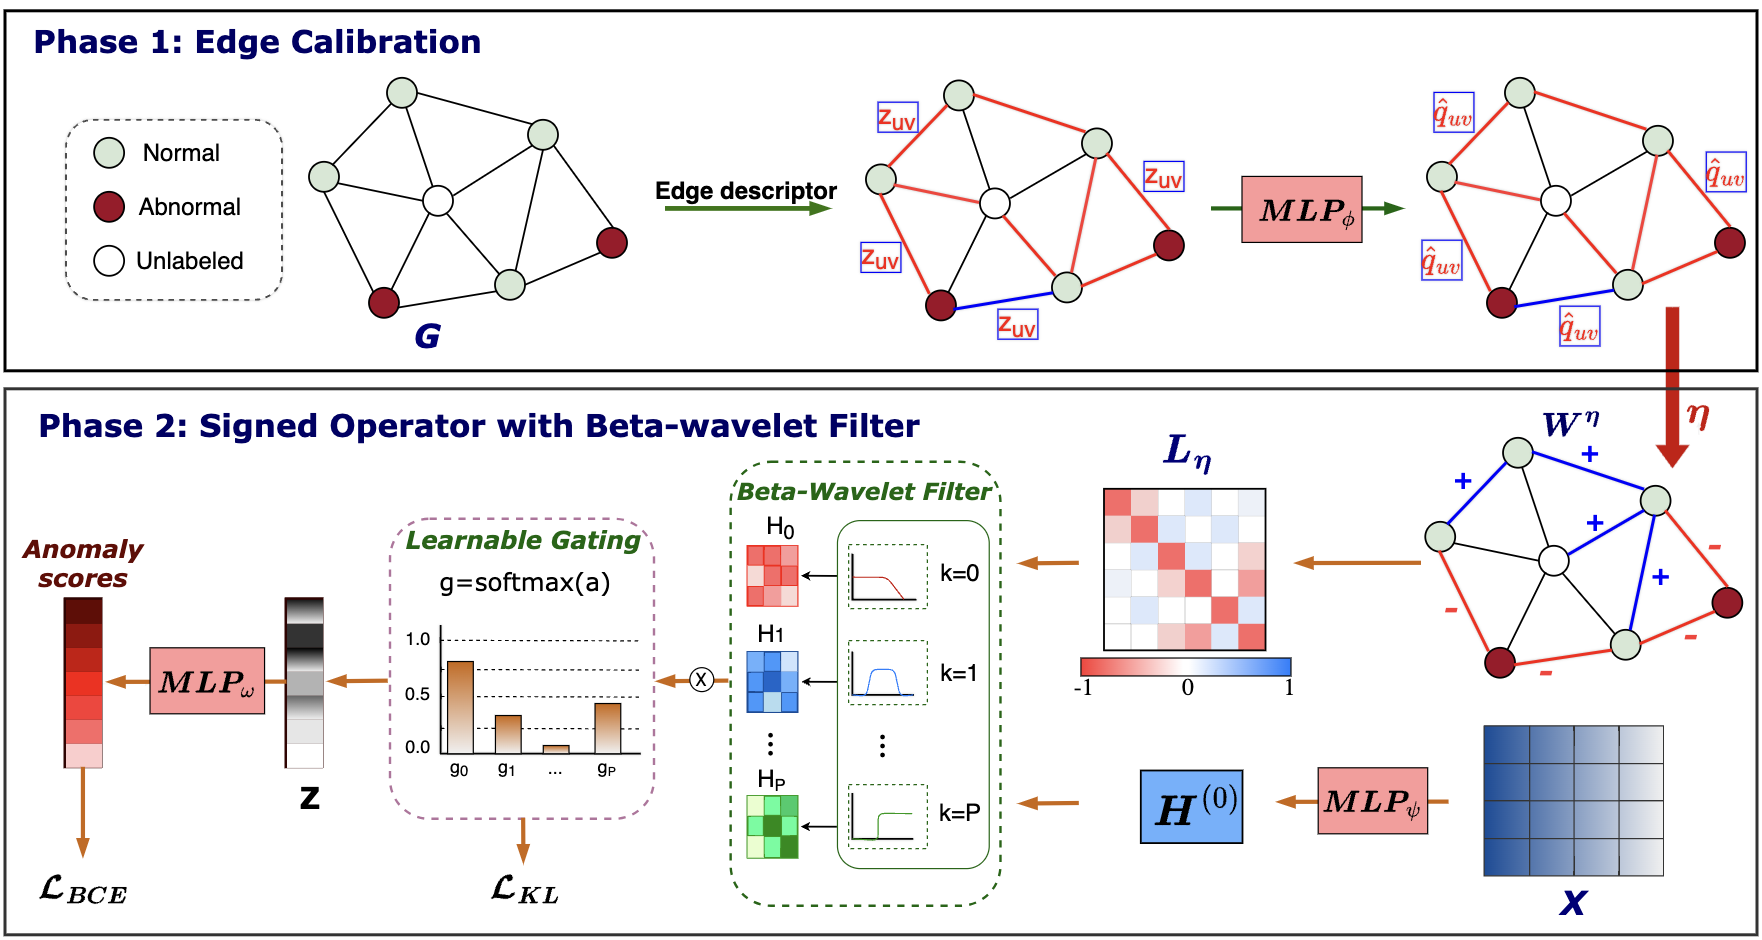
\includegraphics[width=0.9\linewidth]{images/pipeline3.png}}
\caption{Overview of our proposed ESO-GAD with two main phases. The edge calibration phase trains an estimator parameterized by $\phi$ with K-fold cross-fitting to predict the heterophily score $\hat{q}_{uv}$. The second phase constructs a signed spectral operator on the calibrated signed weights and learns to predict the anomaly nodes, with a KL-regularized aggregator.} 
\label{fig:framework}
% \vspace{-10pt}
\end{figure*}
\subsection{Edge Calibration for Heterophily Score Estimation}\label{sec:calibration}
Our main target of ESO-GAD is to include the relational semantics of an edge into the spectral filtering in the frequency domain.
Recent evidence on edge heterophily discrimination shows
that homophilic and heterophilic edges can be estimated from local features~\citep{GREET, H2-FDetector}.
We therefore cast edge-semantics estimation as a supervised task, which classifies edges as heterophilic or homophilic given the input training data.
For each edge $(u,v)\in\cE$ we learn a heterophily probability
\begin{equation}
  q_{uv} \;=\; \Pr\!\left[\, y_u \neq y_v \,\middle|\, \vz_{uv} \,\right]
  \;\in\; [0,1],
  \label{eq:quv}
\end{equation}
where $\vz_{uv}$ is a symmetric edge descriptor and the probability is parameterized by a small multilayer perceptron (MLP).
The probabilistic design is necessary in ESO-GAD because the labeled set $\cV_L$ is tiny and severely imbalanced.
The output probability $q_{uv}$ can be considered as a smooth transition of an edge semantic between the homophily label and heterophily label.
Unlike hard pruning, where each false positive deletes the local structure, a calibrated soft probability is expected to degrade gracefully when there is uncertainty in classifying the edge.

The edge descriptor $\vz_{uv}$ comprises a feature component $\vz^{x}_{uv}$ and a local structural component $\vz^{s}_{uv}$.
Comparing endpoint features is a standard basis for edge representations in various graph learning tasks ~\citep{node2vec,
CARE-GNN, GREET}.
Following this construction, we combine three symmetric similarity measures for the feature similarity component $\vz^{x}_{uv}$ of the edge $(u,v)\in\cE$ with feature vectors $\vx_u, \vx_v \in \mathbb{R}^{d}$:
\begin{equation}
  \vz^{x}_{uv} \;=\;
  \bigl[\, |\vx_u-\vx_v|,\; \vx_u\odot\vx_v,\; \cos(\vx_u,\vx_v) \,\bigr],
  \label{eq:zfeature}
\end{equation}
where $\odot$ is the Hadamard product, $\cos(\cdot,\cdot)$ the cosine similarity, and
$\vz^{x}_{uv}\in\mathbb{R}^{2d+1}$.
Each component of $\vz^{x}_{uv}$ captures complementary semantic information about the relation between the endpoints, which is useful for characterizing how information relevant to the target label propagates along the edge.
%the absolute difference captures attribute disagreement, the Hadamard product captures co-activation patterns.

The structural block $\vz^{s}_{uv}$ collects local statistics of the two end-points, which include
\begin{equation}
\begin{aligned}
  \vz^{s}_{uv} \;=\;
  \Bigl[\,&
    \log(1{+}d_u)+\log(1{+}d_v),\;
    \bigl|\log\tfrac{1+d_u}{1+d_v}\bigr|,\\
    &J_{uv},\;
    \tfrac{|\cN_u\cap\cN_v|}{\sqrt{d_u d_v}}
  \,\Bigr],
\end{aligned}
  \label{eq:structural}
\end{equation}
with $J_{uv}=|\cN_u\cap\cN_v|/|\cN_u\cup\cN_v|$ the Jaccard overlap of the endpoint neighborhoods $\cN_u$, $\cN_v$ .
The symmetric degree sum and absolute log-ratio encode the magnitude and asymmetry of endpoint connectivity, while the
overlap terms measure triadic closure around the edge.
%These quantities are directly motivated by fraud topology 
Given a camouflaged anomaly node, it can be attached to well-connected normal nodes but rarely shares their neighborhoods, so heterophilic edges concentrate at large degree asymmetry and low overlap~\citep{CARE-GNN,PCGNN}.

The complete edge descriptor $\vz_{uv}$ is constructed as 
\begin{equation}
    \vz_{uv} = \Bigl[\,\vz^{x}_{uv} \;\|\; \vz^{s}_{uv} \Bigr],
    \label{eq:zuv}
\end{equation}
where $\|$ is a concatenation operator.
It is clear that $\vz_{uv}$ preserves the symmetric semantic of the edge in this construction and prevents label leakage of the targeted label into the extracted features.
We employ a shallow MLP network, parameterized by $\phi$, to train a prediction function from the input $\vz_{uv}$ to the homophily/heterophily semantic of the edge.
The training target $t_{uv}$ is based on whether the endpoints of an edge $(u, v)$ belong to the set $\mathcal{V}_L$.
Firstly, the edge set is split according to how many of its endpoints belong to the training set $\mathcal{V}_L$:
\begin{align}
  \mathcal{E}_2 &= \{(u,v)\in\mathcal{E} :   |\{u, v\} \cap \mathcal{V}_L| = 2 \} \label{eq:tuvE2}, \\
  \mathcal{E}_1 &= \{(u,v)\in\mathcal{E} : |\{u, v\} \cap \mathcal{V}_L| = 1 \} \label{eq:tuvE1}
\end{align}
and let $\mathcal{E}_0$ collect the remaining edges.
For $(u,v)\in\mathcal{E}_2\cup\mathcal{E}_1$
we assign the binary heterophily target
\begin{equation}
  t_{uv} =
  \begin{cases}
    \mathds{1}\!\left[\, y_u \neq y_v \,\right], & (u,v)\in\mathcal{E}_2,\\[2pt]
    y_u, & (u,v)\in\mathcal{E}_1,\; u \in \mathcal{V}_L,\\[2pt]
    y_v, & (u,v)\in\mathcal{E}_1,\; v \in \mathcal{V}_L .
  \end{cases}
  \label{eq:edge-target}
\end{equation}
The first case is the definition of edge heterophily and it constructs a clean label edge set for training.
The remaining cases are the same definition evaluated under modal imputation of the missing endpoint.
Because anomalies are rare, the marginally most probable label of an unobserved node is
$\hat{y}=0$, and $\mathds{1}[\,y_u \neq 0\,] = y_u$.
A singly-labeled edge is therefore treated as
heterophilic when its labeled endpoint is anomalous and as homophilic otherwise, which is consistent with the camouflage assumption in fraud graphs.
From the empirical aspect, admitting the approximated targets in $\mathcal{E}_1$ trades label noise against the number of training samples.
Nevertheless, it is expected to have a bias estimate of the heterophily target of the edges in $\mathcal{E}$ under the semi-supervised setting.
We deliberately admit this approximation error rather than restricting training to $\mathcal{E}_2$ because the operator is designed to absorb the noisy estimate.
Proposition~\ref{prop:e1} characterizes exactly what the resulting target estimates, and Corollary~\ref{cor:camouflage} states when the imputation is beneficial.

The trained parameters $\phi$ are then used to produce the predicted soft heterophily score
\begin{equation}
  \hat{q}_{uv} \;=\; \text{MLP}_\phi(\vz_{uv})
  \label{eq:quvfromphi}
\end{equation}
The training loss of Phase 1 is designed as
\begin{equation}
    \mathcal{L}_{EC} = \mathcal{L}_{BCE}(t_{uv}, \hat{q}_{uv}) +   \mathcal{L}_{MSE}(t_{uv}, \hat{q}_{uv})
    \label{eq:LossEC}
\end{equation}
where $\mathcal{L}_{BCE}$ and $\mathcal{L}_{MSE}$ are the binary cross entropy loss and the Brier loss, respectively.
The Brier loss is additionally included to encourage calibrated edge-heterophily probabilities, since edge-level predictions in GNNs can exhibit substantial probability miscalibration \citep{nascimento2024innout}.
To reduce the estimation noise caused by the sparsity of the training data, and to keep the labels of a node out of the scores of its own edges, the calibrator is cross-fitted with folds that are grouped by node.
The labeled nodes $\mathcal{V}_L$ are split into $K$ class-stratified folds $\mathcal{F}_1,\dots,\mathcal{F}_K$, and the $j$-th model $\phi^{(j)}$ is trained on the edges of $\mathcal{E}_2\cup\mathcal{E}_1$ none of whose labeled endpoints lies in $\mathcal{F}_j$.
An edge is then scored by the average of the models whose held-out fold contains one of its endpoints, and by the average of all $K$ models when neither endpoint is labeled.
Proposition~\ref{prop:crossfit} states which scores are free of a node's own label under this rule.
%The full training pipeline is given in Algorithm 1.
After getting the aggregated prediction score $\hat{q}_{uv}$, we set $\hat{q}_{uu} = 0$ i.e. the self-loop edge is always homophilic.
%\begin{algorithm}[h]
%\caption{Edge calibration with K-fold training}
%\label{alg:ecsbwgnn}
%\begin{algorithmic}[1]
%\Require Graph $G$, labeled set $\mathcal{V}_L$, folds $K$
%\State Compute the edge descriptor $z_{uv}$ using Eq.~\eqref{eq:zfeature}
%\State Stratify $\mathcal{V}_L$ into $K$ folds
%\For{$j = 1,\dots,K$}
%  \State Construct the target for fold $j$, based Eq.~\eqref{eq:edge-target}
%  \State Train $MLP_\phi^{(j)}$ on using $\mathcal{L}_{EC}$ in Eq.~\eqref{eq:LossEC}
%\EndFor
%\State Average out-of-fold predictions to get $\hat{q}_{uv}$
%\end{algorithmic}
%\end{algorithm}


\subsection{Signed Operator with Beta-wavelet Filter}\label{sec:operator}
The signed operator is designed based on the assumption that the edge semantic can be represented under a signed, continuous value rather than a binary decision.
Given the predicted heterophily score $\hat{q}_{uv}$ in Phase 1, we start by constructing the signed adjacency matrix $\hat{S} = [\hat{s}_{uv}]$ 
\begin{equation}
    \hat{s}_{uv} = 1 - 2 \hat{q}_{uv},
    \label{eq:suv}
\end{equation}
with $\hat{s}_{uv} \in [-1,1]$.
Note that if we know the true value $s_{uv}$ we can easily reconstruct the underlying labels from the training nodes.
However, due to the lack of node labels in semi-supervised settings, we only have a noisy estimate of $s_{uv}$ through $\hat{q}_{uv}$.

To incorporate the uncertainty of heterophilic edge semantics, we introduce a
learned parameter $\eta\in[0,1]$ as the signed weight applied to the self-looped
adjacency matrix $\tilde{\bm A}$,
\begin{equation}
    \bm{W}^{(\eta)} \;=\; \tilde{\bm{A}}\odot\bigl[(1-\eta)\bm{1}\bm{1}^{\!\top}
    + \eta\,\hat{\bm{S}}\bigr],
    \label{eq:weta}
\end{equation}
where $\hat{\bm S}=\bm{1}\bm{1}^{\!\top}-2\hat{\bm Q}$ is the soft sign matrix
induced by the frozen probabilities $\hat{\bm Q}=[\hat q_{uv}]$,
with $\hat q_{uv}=\hat q_{vu}\in[0,1]$ and $\hat q_{uu}\equiv 0$.
Expanding Eq.~\eqref{eq:weta} entrywise gives the scalar form
\begin{equation}
W^{(\eta)}_{uv} \;=\; \tilde A_{uv}\,\bigl(1-2\eta\,\hat q_{uv}\bigr).
\label{eq:Wentry}
\end{equation}
The role of calibration strength $\eta$ is a global gain on the signed correction.
When edge predictions are unreliable, $\eta$ can shrink to $0$ and the operator reduces to the unsigned Laplacian of BWGNN.
ESO-GAD therefore extends BWGNN along the operator axis, providing the same filter bank with a spectrum that carries calibrated edge semantics.
Moreover, the same scalar controls where signs flip.
Since $W^{(\eta)}_{uv}<0$ requires $\hat q_{uv}>1/(2\eta)$, and
since $\hat q_{uv}\le 1$, no edge can change sign unless $\eta>\tfrac12$.
For $\eta\ge\tfrac12$, an edge is exactly pruned when $\hat q_{uv}=1/(2\eta)$.
Because Eq.~\eqref{eq:Wentry} is affine in
$\hat q_{uv}$, no choice of $\eta$ reproduces a thresholded pruning rule, and edge deletion survives only on the measure-zero level set $\{\hat q_{uv}=1/(2\eta)\}$.
This distinguishes ESO-GAD from hard-pruning approaches to heterophily \citep{GHRN, CARE-GNN}, which discard inter-class edges and therefore
receive no gradient signal from them once removed.
By contrast, training $\eta$ jointly with the filters lets the model invert, or restore the contribution of a predicted-heterophilic edge, and every edge retains a gradient path throughout optimization.
Besides the signed weight calibration in Eq.~\eqref{eq:weta}, reweighting approaches such as \citep{SEC-GFD} can be used to construct the operator.
We provide a comparison with pruning and reweighting approaches in the experimental section.

The signed weights $W^{(\eta)}_{uv}$ in Eq.~\eqref{eq:Wentry} break the usual degree normalization due to the possible negative values.
Therefore, we normalize the degree by using the absolute degree \citep{KunegisSigned}:
\begin{equation}
D^{(\eta)}_{uu}=\textstyle\sum_v \bigl|W^{(\eta)}_{uv}\bigr|,
\label{eq:degreelaplacian}
\end{equation}
and create the Laplacian accordingly
\begin{equation}
\Lb \;=\; \bm{I}-\Db{}^{-1/2}\,\Wb\,\Db{}^{-1/2}.
\label{eq:laplacian}
\end{equation}
Its quadratic form decomposes edge-wise as
\begin{equation}
\bm{h}^{\!\top}\Lb\bm{h}
=\tfrac12\sum_{u,v}\bigl|W^{(\eta)}_{uv}\bigr|
\Bigl(\tfrac{h_u}{\sqrt{D^{(\eta)}_{uu}}}-\sgn\!\bigl(W^{(\eta)}_{uv}\bigr)\tfrac{h_v}{\sqrt{D^{(\eta)}_{vv}}}\Bigr)^{\!2},
\label{eq:quadform}
\end{equation}
which smooths across positively signed edges and enforces contrast across negatively signed ones, with per-edge strength $|1-2\eta \hat{q}_{uv}|$.
Heterophilic edges from the calibration phase are retained with reversed semantics rather than discarded like other pruning-based approaches.

Following BWGNN~\citep{BWGNN}, the $k$-th channel applies the Beta-wavelet kernel to $\Lb$, with the spectrum mapped from $[0,2]$ to the Beta support $[0,1]$ as:
\begin{equation}
\Wk(\Lb)
=\frac{1}{2\,\mathrm B(k{+}1,\,P{-}k{+}1)}
\Bigl(\tfrac{\Lb}{2}\Bigr)^{\!k}
\Bigl(\bm I-\tfrac{\Lb}{2}\Bigr)^{\!P-k},
\label{eq:betakernel}
\end{equation}
for $k=0,\dots,P$, giving $P+1$ channels in total.
In Eq.~\eqref{eq:betakernel}, $\mathrm B(\cdot,\cdot)$ is the Beta function, $P$ is the wavelet order and
the factor $\tfrac12$ is the Jacobian of the rescaling.
Under this formulation, the channel $k=0$  and $k=P$ are the low-pass filter and the high-pass filter, respectively.
Intermediate channels cover band-pass responses whose peaks sweep monotonically across the calibrated spectrum.
It is required that the kernel $\Wk(\Lb)$ is valid for any $\Lb$ constructed from the learned $\hat{q}_{uv}$ and a valid $\eta$, which is established by Proposition~\ref{prop:valid}.
\begin{proposition}[Spectral validity]\label{prop:valid}
Let $\tilde{\bm A}=\bm A+\bm I$ and let the scores be symmetric with $\hat q_{uu}=0$. For every such $\hat q\in[0,1]^{|\mathcal E|}$ and every $\eta\ge0$, in particular for every $\eta\in[0,1]$, the following conditions hold
\[
\Db\succeq \bm I \succ 0
\qquad\text{and}\qquad
\lambda_i\in[0,2],
\]
where $\lambda_i$ is an eigenvalue of $\Lb$.
\end{proposition}
%As a result, every Beta-wavelet kernel $\Wk(\Lb)$ of Eq.~\eqref{eq:betakernel} is well defined
In implementation, the product form in Eq.~\eqref{eq:betakernel} is not computed directly.
Instead, each kernel is pre-expanded into monomials of $\Lb$ with fixed coefficients $\theta^{(k)}_j$,
\begin{equation}
\Wk(\Lb)=\sum_{j=0}^{P}\theta^{(k)}_j\,\Lb^{\,j}.
\label{eq:monomial}
\end{equation}
At the first layer, a MLP network with parameters $\psi$ is used to map the input feature space into the initial hidden representation $\bm H^{(0)}= \text{MLP}_\psi(\bm X)$.
Then, every channel
\begin{equation}
\bm H_k=\Wk(\Lb)\,\bm H^{(0)},\qquad k=0,\dots,P,
\label{eq:channels}
\end{equation}
is computed using the fixed coefficients in Eq.~\eqref{eq:monomial}.
%The total computation is evaluated by at most $D$ sparse matrix-vector products
%The powers $\Lb^{\,j}\bm H^{(0)}$ are shared across channels, so the whole bank costs $O(D\,|\mathcal E|\,d)$ per forward pass.

Because $\eta$ is trained jointly with the filters, Eq.~\eqref{eq:weta} and Eq.~\eqref{eq:laplacian} are re-evaluated at every forward pass, which makes the filter bank a moving operator, and only at convergence is there one fixed $\Lb$ per dataset.
A small update of $\eta$ would introduce stochasticity into the underlying operator.
In order to improve the stability of the training process, we design an anchored gate in the later weighted aggregation $\bm H_k$ to produce the output latent representation.
An additional KL loss is added to prevent the collapse issue when the signal is not informative at the start of the training phase.
Specifically, the channel outputs are combined by a learnable simplex gate $\bm{g}=\mathrm{softmax}(\bm{a})$:
\begin{equation}
\bm{Z}=\big\Vert_{k=0}^{P}\sqrt{g_k}\,\bm{H}_k,
\label{eq:gate}
\end{equation}
 where $\bm{a}$ is trainable.
The classification output head $\text{MLP}_\omega$ is then used to map to the target label as:
\begin{equation}
\hat{\bm{y}}= \text{MLP}_\omega(\bm{Z}).
\end{equation}
Given the set of available labels $\bm{y}^L$ and the predicted output $\hat{\bm{y}}^L$, the whole module is  trained with
\begin{equation}
\mathcal{L}
=\mathcal{L}_{\mathrm{BCE}}(\bm{y}^L,\hat{\bm{y}}^L)
+\alpha\, D_{\mathrm{KL}}\!\bigl(\bm{g}\,\Vert\,\bm{g}_0\bigr),
\label{eq:loss}
\end{equation}
where $\bm{g}_0$ is the uniform prior and $\alpha$ is the weighting coefficient.
The gate acts as an adaptive frequency response for readout procedure.
The learned $\bm{g}$ decides which signed-spectral bands carry anomaly evidence on a given dataset, replacing the standard Beta-wavelet's fixed concatenation.
By combining the gate with the KL loss, it stabilizes training under a moving operator.
The pseudocode of ESO-GAD is presented in Algorithm~\ref{alg:ecsbwgnn}.

The runtime complexity of ESO-GAD combines two phases.
In the first phase, with $n=|\mathcal V|$, $m=|\mathcal E|$ and edge-descriptor dimension $d_e$, the training cost for each fold is approximately $O(m\,d_e)$, which is linear in the number of edges.
In Phase~2, each forward pass rebuilds $\bm W^{(\eta)}$ and
$\bm D^{(\eta)}$ from the frozen $\hat{\bm Q}$ in $O(m)$ time and shares the powers $\bm L_\eta^{\,j}\bm H^{(0)}$ across all $P{+}1$ channels via Eq.~\eqref{eq:monomial}.
This results in a per-epoch cost of
$O\bigl(P\,m\,d_h+P^{2}n\,d_h\bigr)$ with the hidden width $d_h$ of both $\psi$ and $\omega$.
The cost matches the standard Beta-wavelet bank~\citep{BWGNN}.
The coefficients $\theta^{(k)}_j$ are constants that do not depend on $\eta$; what changes with $\eta$ is the operator, which is rebuilt at every step in $O(m)$ time, whereas the unsigned bank builds its operator once. This additional cost is dominated by the $O(P\,m\,d_h)$ propagation by a factor of $P\,d_h$.

\begin{algorithm}[h]
\caption{ESO-GAD training}
\label{alg:ecsbwgnn}
\begin{algorithmic}[1]
\REQUIRE Graph $G$, labeled set $\mathcal{V}_L$ with labels $y_L$, wavelet order $P$, predicted score matrix $\hat{\bm Q}=[\hat q_{uv}]$
%\STATE Initialize $\eta$, gate logits $a$, encoder paramters $\theta$, and classifier parameters $\omega$
\FOR{epochs=$1,\dots$}
  \STATE $\hat s_{uv} \gets 1-2\hat{q}_{uv}$
  \STATE Compute $W^{(\eta)}$ and $D^{(\eta)}$ using Eqs.~\eqref{eq:weta} and~\eqref{eq:degreelaplacian}
  \STATE $L_\eta \gets I - D^{(\eta)-1/2}W^{(\eta)}D^{(\eta)-1/2}$
  \STATE $\bm H^{(0)} \gets \text{MLP}_\psi(X)$
  \FOR{$k=0,\dots,P$}
    \STATE $\bm H_k \gets \Wk(\Lb)\,\bm H^{(0)}$
  \ENDFOR
  \STATE $\bm{g} \gets \mathrm{softmax}(\bm{a})$; $\bm Z \gets \big\Vert_{k=0}^{P}\sqrt{g_k}\,\bm{H}_k$
  \STATE $\hat{\bm{y}} \gets \text{MLP}_\omega(Z)$
  \STATE $\mathcal L \gets \mathcal{L}_{\mathrm{BCE}}(\bm{y}^L,\hat{\bm{y}}^L) +\alpha\, D_{\mathrm{KL}}\!\bigl(\bm{g}\,\Vert\,\bm{g}_0\bigr)$
  \STATE Update $(\psi,\omega,\eta,a)$ on $\mathcal L$
\ENDFOR
\end{algorithmic}
\end{algorithm}

\section{Theoretical Analysis}\label{sec:theory}
% Section "Theoretical Analysis". All proofs are in proof.tex (Appendix A).
% Each statement has a numerical check in src/theory_check.py; keep the two in sync.
The construction of Section~\ref{sec:method} raises three questions that an empirical comparison alone cannot settle: why a signed operator should separate anomalies better than an unsigned one, why the estimated edge semantics should enter as signs rather than through pruning or reweighting, and how far the errors of a frozen calibrator can propagate.
This section answers them in turn.
Section~\ref{sec:theory-spectral} locates the label signal in the spectrum of $\Lb$.
Section~\ref{sec:theory-node} analyzes separability at node level and derives the optimal edge weights.
Section~\ref{sec:theory-supervision} characterizes what the weak edge supervision of Phase~1 identifies.
Section~\ref{sec:theory-stability} bounds the effect of calibration errors on the operator and on the representation.
All proofs are deferred to Appendix~\ref{app:proofs}.

\paragraph{Notation.}
For the analysis we write the labels in signed form, $\bar y_u=2y_u-1\in\{-1,+1\}$, with $\ys$ the signed label vector and $\Ys=\operatorname{diag}(\ys)$.
The true heterophily indicator of an edge is $\tstar_{uv}=\mathds{1}[y_u\neq y_v]$, collected in $\bm t^\star$, and its true sign is $\sstar_{uv}=\bar y_u\bar y_v=1-2\tstar_{uv}$, with $\sstar_{uu}=1$.
A \emph{score vector} $q\in[0,1]^{|\mathcal E|}$ is any symmetric assignment of scores to the edges with $q_{uu}=0$.
We write $\bm L_\eta(q)$ for the Laplacian of Eq.~\eqref{eq:laplacian} built from $q$ and $\eta$, $W_{uv}$ and $D_{uu}$ for the entries of the corresponding $\Wb$ and $\Db$, and $\sigma_{uv}=\sgn(W_{uv})$.
Sums over $(u,v)$ run over ordered pairs with $\tilde A_{uv}=1$, self-loops included, and $\tilde d_u=\sum_v\tilde A_{uv}$.
The local heterophily of a node is $\tilde h_u=\tilde d_u^{-1}\sum_v\tilde A_{uv}\tstar_{uv}$, and $\tilde h_a$, $\tilde h_n$ are its averages over anomalous and normal nodes.
Finally,
\begin{equation}
\kappa_k=\frac{1}{2\,\mathrm B(k{+}1,\,P{-}k{+}1)}=\frac{P{+}1}{2}\binom{P}{k}
\label{eq:kappa}
\end{equation}
denotes the prefactor of the $k$-th Beta kernel in Eq.~\eqref{eq:betakernel}.
Unless stated otherwise, the results hold for every $\eta\ge0$, which includes the range $[0,1]$ used by ESO-GAD.

%%%%%%%%%%%%%%%%%%%%%%%%%%%%%%%%%%%%%%%%%%%%%%%%%%%%%%%%%%%%%%%%%%%%%%%%%%%%%%%%
\subsection{Why Signing Helps: Balance and Label Frequency}\label{sec:theory-spectral}

We first ask what the operator does when the edge semantics are known exactly.

\begin{theorem}[Oracle signs are a change of gauge]\label{thm:gauge}
Let $q=\bm t^\star$ and $\eta\in[\tfrac12,1]$. Then:

\smallskip\noindent\textbf{(i)} $\bm L_\eta(\bm t^\star)=\Ys\,\bm L_{1-\eta}(\bm t^\star)\,\Ys$, where all edge weights of $\bm L_{1-\eta}(\bm t^\star)$ are non-negative and $\bm L_{0}$ is the unsigned operator of BWGNN.

\smallskip\noindent\textbf{(ii)} $\bm L_\eta(\bm t^\star)$ and $\bm L_{1-\eta}(\bm t^\star)$ have the same spectrum, and $g(\bm L_\eta(\bm t^\star))=\Ys\,g(\bm L_{1-\eta}(\bm t^\star))\,\Ys$ for every polynomial $g$, in particular for every Beta kernel $\Wk$.

\smallskip\noindent\textbf{(iii)} $\bm L_\eta(\bm t^\star)\,\Db{}^{1/2}\ys=\bm 0$.
\end{theorem}

Filtering with the oracle signed operator is therefore the same as flipping the features of one class, filtering on a graph in which every edge is homophilic, and flipping back.
Signing leaves the spectrum untouched and moves the label signal to frequency zero.
Pruning also reaches frequency zero, but on a smaller graph; Section~\ref{sec:theory-node} quantifies the difference.
Theorem~\ref{thm:gauge} specializes structural balance~\citep{Harary1953} and switching equivalence~\citep{Zaslavsky1982,KunegisSigned} to the $\eta$-family of Eq.~\eqref{eq:weta}.
It relies on the fact that, for two classes, the product of the true signs along any walk from $u$ to $v$ equals $\bar y_u\bar y_v$.
With three or more classes the label-induced signs are in general not balanced, and signed message passing is known to update multi-hop neighbors undesirably in that case~\citep{SignNotRemedy}.
Binary anomaly detection is the setting in which this issue cannot arise under correct signs.

For an arbitrary calibrator, the relevant quantity is how much edge weight carries the wrong sign.
We define the \emph{frustration} of the signed graph with respect to the labels and the frequency of the \emph{label signal} $\yt=\Db{}^{1/2}\ys$ as
\begin{align}
\Fr_\eta(q)&=\frac{\sum_{u,v}|W_{uv}|\,\mathds{1}[\sigma_{uv}\neq\sstar_{uv}]}{\sum_{u,v}|W_{uv}|},\label{eq:frustration}\\
\rho_\eta(q)&=\frac{\yt^{\top}\bm L_\eta(q)\,\yt}{\yt^{\top}\yt}.\label{eq:labelfreq}
\end{align}

\begin{theorem}[Label frequency equals frustration]\label{thm:freq}
For every graph, every labeling, every score vector $q$ and every $\eta\ge0$,
\[
\rho_\eta(q)=2\,\Fr_\eta(q).
\]
\end{theorem}

Theorem~\ref{thm:freq} ties the quality of the calibrator directly to the spectrum: signing lowers the frequency of the label signal exactly as far as the signs are right.
Bounds between the least eigenvalue of a signed Laplacian and its frustration are classical~\citep{Belardo2014,AtayLiu2020}; the identity above concerns the label partition and holds for every calibration strength.

\begin{corollary}[Unsigned and reweighting regimes]\label{cor:lift}
Let $H$ be the number of heterophilic ordered edges, $M$ the number of all ordered edges including self-loops, and $S_{\mathrm{het}}$, $S_{\mathrm{all}}$ the sums of $q_{uv}$ over these two sets.
For $\eta\in[0,\tfrac12]$,
\[
\Fr_\eta(q)=\frac{H-2\eta S_{\mathrm{het}}}{M-2\eta S_{\mathrm{all}}}.
\]
In particular, $\rho_0=2H/M$ is twice the edge heterophily ratio, and $\Fr_\eta(q)$ is strictly decreasing in $\eta$ on $[0,\tfrac12]$ if and only if $S_{\mathrm{het}}/H>S_{\mathrm{all}}/M$.
\end{corollary}

At $\eta=0$ the frequency of the label signal is the edge heterophily ratio, which recovers in one line the link between heterophily and high-frequency energy behind the right-shift of BWGNN~\citep{BWGNN} and behind GHRN~\citep{GHRN}.
The second statement says that every calibrator with positive lift, i.e., whose mean score on heterophilic edges exceeds its mean score on all edges, lowers the label frequency throughout the reweighting regime.
For $\eta>\tfrac12$ edges start to flip, and
\[
\Fr_\eta(q)=\frac{\sum_{\mathrm{het}}(1-2\eta q_{uv})_+ +\sum_{\mathrm{hom}}(2\eta q_{uv}-1)_+}{\sum_{\mathrm{all}}|1-2\eta q_{uv}|},
\]
which rewards correct flips and charges wrong ones.

\begin{corollary}[Label energy across channels]\label{cor:energy}
Let $E_k=\|\Wk(\bm L_\eta(q))\,\yt\|_2^2/(\kappa_k^2\|\yt\|_2^2)$ be the share of label energy passed by channel $k$. Then
\begin{align*}
\bigl(1-\Fr_\eta(q)\bigr)^{2P}&\le E_0\le 1-\Fr_\eta(q),\\
\Fr_\eta(q)^{2P}&\le E_P\le\Fr_\eta(q).
\end{align*}
\end{corollary}

The signed operator thus moves label energy from the high-pass channel to the low-pass channel in proportion to the frustration it removes.
Under oracle signs, $E_0=1$ and $E_k=0$ for $k\ge1$.
This is the precise sense in which signing reallocates frequency, and it gives the gate of Eq.~\eqref{eq:gate} a concrete role: the better the calibration, the more label energy sits in the low channels.

%%%%%%%%%%%%%%%%%%%%%%%%%%%%%%%%%%%%%%%%%%%%%%%%%%%%%%%%%%%%%%%%%%%%%%%%%%%%%%%%
\subsection{Sign, Reweight, or Prune: Node-Level Separability}\label{sec:theory-node}

The spectral view does not distinguish signing from pruning, since both can remove frustration.
The difference appears at node level, where the question is how much evidence about its own class a node receives from its neighbors.

\begin{assumption}[Class-centred features]\label{ass:features}
$\bm H^{(0)}=\ys\bm\mu^{\top}+\bm\Xi$, where $\bm\mu\in\mathbb R^{d_h}$ and the rows of $\bm\Xi$ are i.i.d.\ $\mathcal N(\bm 0,\sigma^2\bm I)$ and independent of the graph and of the scores.
\end{assumption}

This is the feature model of contextual stochastic block models~\citep{CSBM,GCTheory}, imposed on the encoder output and conditional on an arbitrary graph.
For a node $u$ we define the \emph{margin} and the \emph{effective degree}
\begin{equation}
\mar_u=\frac{\sum_vW_{uv}\,\sstar_{uv}}{\sum_v|W_{uv}|},\qquad
\deff_u=\frac{\bigl(\sum_v|W_{uv}|\bigr)^2}{\sum_vW_{uv}^2}.
\label{eq:margin}
\end{equation}
The margin is the correctly signed minus the wrongly signed share of the edge weight of $u$, and $\deff_u\in[1,\tilde d_u]$ counts how many neighbors effectively contribute.

\begin{theorem}[Node-level separability]\label{thm:snr}
Let Assumption~\ref{ass:features} hold, let $\bm G\in\mathbb R^{n\times n}$ depend on $(\tilde{\bm A},q,\eta)$ only, and let $\bm Z=\bm G\bm H^{(0)}$ with rows $\bm z_u$.

\smallskip\noindent\textbf{(a)} The readout $\sgn\langle\bm z_u,\bm\mu\rangle$ misclassifies node $u$ with probability $\Gt\bigl(\snr_u(\bm G)\,\|\bm\mu\|/\sigma\bigr)$, where $\Gt$ is the standard Gaussian tail function and
\[
\snr_u(\bm G)=\frac{\bar y_u\,[\bm G\ys]_u}{\|\bm G_{u\cdot}\|_2}.
\]
For one propagation step, $\bm G=\Db{}^{-1}\Wb$, we have $\snr_u(\bm G)=\mar_u\sqrt{\deff_u}$.

\smallskip\noindent\textbf{(b)} For one step with oracle edge information, $\snr_u$ equals $(1-2\tilde h_u)\sqrt{\tilde d_u}$ for the unsigned operator, $\sqrt{(1-\tilde h_u)\,\tilde d_u}$ for pruning ($W_{uv}=\tilde A_{uv}(1-\tstar_{uv})$), and $\sqrt{\tilde d_u}$ for signing ($W_{uv}=\tilde A_{uv}(1-2\tstar_{uv})$).

\smallskip\noindent\textbf{(c)} Let $g$ be a polynomial with non-negative coefficients, $\bm G_0=g(\bm I-\bm L_0)$ and $\bm G_s=g(\bm I-\bm L_1(\bm t^\star))$. Then for every node $u$,
\[
\snr_u(\bm G_s)=\frac{\|\bm G_{0,u\cdot}\|_1}{\|\bm G_{0,u\cdot}\|_2}\;\ge\;|\snr_u(\bm G_0)|,
\]
with strict inequality if and only if the support of row $u$ of $\bm G_0$ contains both classes.

\smallskip\noindent\textbf{(d)} For $\bm G=\Db{}^{-1}\Wb$,
\[
\frac{d\snr_u}{d\eta}\Big|_{\eta=0}
=4\sqrt{\tilde d_u}\;\tilde h_u(1-\tilde h_u)\bigl(\bar q^{\mathrm{het}}_u-\bar q^{\mathrm{hom}}_u\bigr),
\]
where $\bar q^{\mathrm{het}}_u$ and $\bar q^{\mathrm{hom}}_u$ are the mean scores on the heterophilic and homophilic edges of $u$, the self-loop counting as homophilic with score $0$.
\end{theorem}

Part~(b) separates the three ways of using edge semantics.
Signing and pruning both place a node on the side of its own class, but pruning discards the heterophilic neighbors while signing keeps them as evidence, so $\snr^{\mathrm{sign}}_u/\snr^{\mathrm{prune}}_u=(1-\tilde h_u)^{-1/2}$, which is largest for camouflaged anomalies.
The unsigned operator places every node with $\tilde h_u>\tfrac12$ on the wrong side.
Averaging $[\bm G\ys]_u=\mar_u\bar y_u$ over each class shows that one unsigned step separates the class means by $2\,|1-\tilde h_a-\tilde h_n|\,\|\bm\mu\|$, against $2\|\bm\mu\|$ for oracle signing.
In the camouflage regime, where anomalies are mostly linked to normal nodes ($\tilde h_a$ close to $1$, $\tilde h_n$ close to $0$), the two class means collapse onto each other.
An unsigned high-pass filter does keep every node on its own side, since $\bar y_u[(\bm I-\tilde{\bm D}^{-1}\tilde{\bm A})\ys]_u=2\tilde h_u$ with $\tilde{\bm D}$ the degree matrix of $\tilde{\bm A}$, but it does not average the noise, since the corresponding row has squared norm $1-1/\tilde d_u$, so $\snr_u\approx2\tilde h_u\le2$.
The signed low-pass channel reaches $\sqrt{\tilde d_u}$.
Unsigned spectral detectors can therefore see the anomaly signal in the high frequencies but cannot denoise it, whereas signing turns heterophilic neighbors into denoising evidence.
Part~(c) extends the comparison beyond one step: the low-pass Beta kernel $\mathcal W_0\propto(\bm I-\Lb/2)^P$ has the required form, and under oracle signs it dominates its unsigned counterpart at every node.
Part~(d) shows that any calibrator that ranks the heterophilic edges of a node above its homophilic ones improves that node at first order, independently of the base rate of heterophily.

\begin{remark}[Scope]\label{rem:scope}
Parts (b) and (d) concern one propagation step and part (c) concerns non-negative filters with a linear readout.
A multi-channel unsigned bank followed by an MLP can combine low-pass and high-pass channels non-linearly, so Theorem~\ref{thm:snr} does not state that an unsigned bank cannot separate the classes.
It states what a single signed low-pass channel achieves that no unsigned channel does.
\end{remark}

\begin{remark}[Two pathways]\label{rem:pathways}
If the encoder output carries a class-independent offset, $\bm H^{(0)}=\bm 1\bm\mu_0^{\top}+\ys\bm\mu^{\top}+\bm\Xi$, one step maps the offset of node $u$ to $\nu_u\bm\mu_0$ with $\nu_u=\sum_vW_{uv}/\sum_v|W_{uv}|$.
For the unsigned operator $\nu_u\equiv1$.
For the signed operator $\nu_u$ summarizes how much of the neighborhood of $u$ is flagged as heterophilic, which is itself informative about the class.
The signed operator thus acts through a \emph{contrast} pathway, analyzed in Theorem~\ref{thm:snr}, and a \emph{bias} pathway that injects a neighborhood summary of the edge scores.
\end{remark}

We now ask which edge weights are best when the edge semantics are uncertain.

\begin{assumption}[Reliability of the scores]\label{ass:reliability}
Conditionally on the scores, the relative signs $\bar y_u\bar y_v$ of the neighbors $v\neq u$ of a node $u$ are independent, and $\Pr[y_u\neq y_v\mid q]=p(q_{uv})$ for a function $p:[0,1]\to[0,1]$, the \emph{reliability curve} of the calibrator.
\end{assumption}

The calibrator is calibrated when $p(q)=q$.

\begin{theorem}[Optimal edge weights]\label{thm:optimal}
Let Assumption~\ref{ass:reliability} hold, and let Assumption~\ref{ass:features} hold with arbitrary independent noise of zero mean and covariance $\sigma^2\bm I$.
Fix a node $u$ and aggregate $\bm z_u=\sum_v\vartheta_v\bm h^{(0)}_v$ over its neighbors in $\tilde{\bm A}$ with weights $\vartheta_v$ that depend on the scores only.
Let $c_v=1-2p(q_{uv})$ for $v\neq u$, $c_u=1$, and $\varsigma_v^2=\sigma^2+\|\bm\mu\|^2(1-c_v^2)$.
With $\hat{\bm\mu}=\bm\mu/\|\bm\mu\|$ and moments taken conditionally on $y_u$ and the scores, the deflection
\[
\mathcal J(\bm\vartheta)
=\frac{\mathbb E\bigl[\bar y_u\langle\bm z_u,\hat{\bm\mu}\rangle\bigr]}{\operatorname{sd}\bigl[\langle\bm z_u,\hat{\bm\mu}\rangle\bigr]}
\]
equals $\|\bm\mu\|\sum_v\vartheta_vc_v\big/\bigl(\sum_v\vartheta_v^2\varsigma_v^2\bigr)^{1/2}$, and:

\smallskip\noindent\textbf{(i)} $\mathcal J(\bm\vartheta)\le\mathcal J^\star=\|\bm\mu\|\bigl(\sum_vc_v^2/\varsigma_v^2\bigr)^{1/2}$, with equality if and only if $\vartheta_v\propto c_v/\varsigma_v^2$.

\smallskip\noindent\textbf{(ii)} Over non-negative weights, $\mathcal J(\bm\vartheta)\le\mathcal J^\star_+=\|\bm\mu\|\bigl(\sum_v(c_v)_+^2/\varsigma_v^2\bigr)^{1/2}$, with equality if and only if $\vartheta_v\propto(c_v)_+/\varsigma_v^2$.

\smallskip\noindent\textbf{(iii)} $(\mathcal J^\star)^2-(\mathcal J^\star_+)^2=\|\bm\mu\|^2\sum_{v:\,p(q_{uv})>1/2}c_v^2/\varsigma_v^2$.

\smallskip\noindent\textbf{(iv)} If $\mathcal J(\bm\vartheta)>0$, the readout $\sgn\langle\bm z_u,\bm\mu\rangle$ errs with probability at most $1/(1+\mathcal J(\bm\vartheta)^2)$.
\end{theorem}

The optimal weight is an odd, increasing function of the soft sign $c_v=1-2p(q_{uv})$.
In the regime where aggregation matters most, $\|\bm\mu\|\ll\sigma$, it is exactly proportional to $1-2p(q_{uv})$, and for confident edges, $|c_v|\to1$, it equals $c_v$ at every signal level.
The unsigned operator ($\vartheta_v\equiv1$), reweighting ($\vartheta_v=1-q_{uv}$) and pruning ($\vartheta_v=\mathds{1}[q_{uv}<\tau]$) use non-negative weights, so they are bounded by $\mathcal J^\star_+$.
By part~(iii), what they lose is exactly the information carried by the edges that are more likely heterophilic than not.
For a fully camouflaged node, $(\mathcal J^\star_+)^2$ retains only the self term, while $(\mathcal J^\star)^2$ grows with the degree.
Theorem~\ref{thm:optimal} also explains why calibration matters beyond ranking quality: the weight that enters is the true posterior, so a miscalibrated score yields suboptimal weights even when its ordering of the edges is perfect.

\begin{corollary}[The calibration strength is a recalibration slope]\label{cor:slope}
Suppose the frozen scores have a linear reliability curve, $p(q)=\eta_0\,q$ with $0\le\eta_0\le1/\max_{u,v}\hat q_{uv}$.
As $\|\bm\mu\|/\sigma\to0$, the optimal weights of Theorem~\ref{thm:optimal} at every node $u$ converge, up to a positive factor, to $\vartheta_v=1-2\eta_0\hat q_{uv}$, i.e., to the row of $\bm W^{(\eta_0)}$.
\end{corollary}

Although the calibrator is frozen after Phase~1, $\eta$ is therefore more than a damping factor.
It is the one-parameter recalibration under which the family of Eq.~\eqref{eq:Wentry} contains the optimal aggregator.
A slope $\eta_0<1$ means that the scores over-predict heterophily, which is the expected case when the labeled set over-represents anomalies or when the edge loss is class-weighted.
A single scalar repairs a linear miscalibration only; scores that are non-monotone in the true posterior, or wrong on a specific type of edge, are beyond its reach.
Proposition~\ref{prop:valid} holds for every $\eta\ge0$, so the theory does not require the slope to stay below one.

%%%%%%%%%%%%%%%%%%%%%%%%%%%%%%%%%%%%%%%%%%%%%%%%%%%%%%%%%%%%%%%%%%%%%%%%%%%%%%%%
\subsection{What Weak Edge Supervision Identifies}\label{sec:theory-supervision}

Theorem~\ref{thm:optimal} calls for the posterior heterophily probability of Eq.~\eqref{eq:quv}, which we write $q^\star(\bm z)=\Pr[y_u\neq y_v\mid\vz_{uv}=\bm z]$.
With few labels, most of the supervision comes from the singly-labeled edges $\mathcal E_1$, whose targets in Eq.~\eqref{eq:edge-target} impute the unlabeled endpoint as normal.
Let $P_{aa}(\bm z)$ and $P_{nn}(\bm z)$ be the probabilities that both endpoints of an edge with descriptor $\bm z$ are anomalous, respectively normal, so that $P_{aa}+P_{nn}+q^\star=1$.

\begin{assumption}[Label sampling]\label{ass:sampling}
Whether a node is labeled depends on its class only: anomalies are labeled with probability $r_1$ and normal nodes with probability $r_0$, independently of each other, of the graph and of the features.
\end{assumption}

\begin{proposition}[Target of singly-labeled edges]\label{prop:e1}
Under Assumption~\ref{ass:sampling}, for an edge of $\mathcal E_1$ with descriptor $\bm z$ and target $t_{uv}$ from Eq.~\eqref{eq:edge-target},
\[
\frac{\Pr[t_{uv}=1\mid\bm z]}{\Pr[t_{uv}=0\mid\bm z]}
=\frac{r_1\bigl[2(1-r_1)P_{aa}+(1-r_0)\,q^\star\bigr]}{r_0\bigl[2(1-r_0)P_{nn}+(1-r_1)\,q^\star\bigr]},
\]
with $P_{aa}$, $P_{nn}$, $q^\star$ evaluated at $\bm z$.
In particular, if $r_1=r_0$ then $\mathbb E[t_{uv}\mid\bm z]=\iota(\bm z):=\tfrac12q^\star(\bm z)+P_{aa}(\bm z)$, and in general the odds equal $\tfrac{r_1}{r_0}\cdot\tfrac{\iota(\bm z)}{1-\iota(\bm z)}$ up to a factor in $[1-r,\,(1-r)^{-1}]$ with $r=\max(r_0,r_1)$.
\end{proposition}

The singly-labeled target therefore ranks edges by $\iota(\bm z)$, the probability that the edge \emph{touches an anomaly}, and not by heterophily: an edge between two anomalies is homophilic but attains the largest $\iota$.
When anomalies are rare and camouflaged, $P_{aa}\approx0$ and $\iota\approx q^\star/2$, a rescaled heterophily probability whose scale the calibration strength absorbs (Corollary~\ref{cor:slope}).
The modal imputation of Eq.~\eqref{eq:edge-target} is thus exact under pure camouflage and biased where anomalies link to each other.

\begin{corollary}[When the imputation helps]\label{cor:camouflage}
Consider the idealized operator that the target of Proposition~\ref{prop:e1} induces at $\eta=1$, in which exactly the edges incident to an anomaly are negative.
Its margin is $\mar_u=1$ for every normal node and $\mar_u=2\tilde h_u-1+2/\tilde d_u$ for every anomaly, against $1-2\tilde h_u$ for the unsigned operator.
Hence it improves the margin of an anomaly $u$ if and only if $\tilde h_u>\tfrac12-\tfrac{1}{2\tilde d_u}$.
\end{corollary}

Corollary~\ref{cor:camouflage} makes the camouflage assumption behind Eq.~\eqref{eq:edge-target} checkable on any dataset through the local heterophily of its anomalies.
Restricting the supervision to $\mathcal E_2$ is not an alternative under the label budget of GADBench: with $100$ labeled nodes, the expected number of doubly-labeled edges is $|\mathcal E|\cdot\tfrac{100\cdot99}{n(n-1)}$, which ranges from about $300$ on Amazon to fewer than one on Questions (Table~\ref{tab:e2size} in Appendix~\ref{app:proofs}).
The bias of the modal imputation disappears when the unlabeled endpoint is instead imputed in expectation, $t_{uv}=y_u(1-\hat p_v)+(1-y_u)\hat p_v$ with $\hat p_v$ a calibrated anomaly probability of the unlabeled endpoint $v$; Eq.~\eqref{eq:edge-target} is the special case $\hat p_v\equiv0$.

The second property of Phase~1 that the analysis relies on is that the scores of a node's edges are produced without that node's label.

\begin{proposition}[Label-free scores under node-grouped cross-fitting]\label{prop:crossfit}
Let the labeled nodes be partitioned into folds $\mathcal F_1,\dots,\mathcal F_K$, let model $\phi^{(j)}$ be trained on the edges none of whose labeled endpoints lies in $\mathcal F_j$, and let an edge be scored by the average of the models $\phi^{(j)}$ whose fold $\mathcal F_j$ contains one of its endpoints, or by all $K$ models if neither endpoint is labeled.
For a labeled node $u\in\mathcal F_a$ and a neighbor $v$:

\smallskip\noindent\textbf{(i)} If $v$ is unlabeled or $v\in\mathcal F_a$, then $\hat q_{uv}$ is a function of the graph, the features and the labels outside $\mathcal F_a$. In particular it does not depend on $y_u$.

\smallskip\noindent\textbf{(ii)} If $v\in\mathcal F_b$ with $b\neq a$, then $\hat q_{uv}$ averages $\phi^{(a)}$ and $\phi^{(b)}$, and $\phi^{(b)}$ is trained with $y_u$.

\smallskip\noindent If cross-fold pairs are instead scored by a model trained without $\mathcal F_a\cup\mathcal F_b$, then no score of an edge incident to $u$ depends on $y_u$.
\end{proposition}

Under the label budget of GADBench, the edges of case~(ii) make up a fraction of about $|\mathcal V_L|/n$, below one percent, of the edges of a labeled node, so the scores that enter the node loss are out-of-sample up to that fraction.
This matters for the calibration strength.
By Corollary~\ref{cor:slope}, $\eta$ estimates the reliability slope of the scores, and it is fitted on the labeled nodes.
In-sample scores would be sharper on the labeled nodes than on the test nodes and would bias this estimate, which is the role sample splitting plays in double machine learning~\citep{DML}.

%%%%%%%%%%%%%%%%%%%%%%%%%%%%%%%%%%%%%%%%%%%%%%%%%%%%%%%%%%%%%%%%%%%%%%%%%%%%%%%%
\subsection{Robustness to Calibration Error}\label{sec:theory-stability}

There are two sources of error in training ESO-GAD.
The scores of Phase~1 are estimates, so their errors enter $\Lb$.
Moreover, because $\eta$ is updated at every step, $\Lb$ is a \emph{moving} operator, and training is stable only if the operator is Lipschitz in the quantities that move.
We measure the discrepancy between two score vectors $q$ and $q'$ locally, through the mean absolute and mean squared errors on the edges of each node,
\begin{align}
\bar e_u&=\frac{1}{\tilde d_u}\sum_v\tilde A_{uv}\,|q_{uv}-q'_{uv}|,&\eloc(q,q')&=\max_u\bar e_u,\notag\\
b_u&=\frac{1}{\tilde d_u}\sum_v\tilde A_{uv}\,(q_{uv}-q'_{uv})^2,&\mathcal B(q,q')&=\sum_ub_u,
\label{eq:localerrors}
\end{align}
and we let $\gamma=\min_uD^{(\eta)}_{uu}(q)/\tilde d_u\in(0,1]$ be the smallest share of a node's edge mass that survives calibration.

\begin{theorem}[Degree-free stability of the operator]\label{thm:stab}
Let $\bm L=\bm L_\eta(q)$ and $\bm L'=\bm L_{\eta'}(q')$ with weights $W_{uv}$, $W'_{uv}$, and let
\[
\delta=\max_u\frac{\sum_v|W_{uv}-W'_{uv}|}{D_{uu}}.
\]
Then
\begin{equation}
\bigl\|\bm L-\bm L'\bigr\|_2\;\le\;3\delta+\delta^2,
\label{eq:stabjoint}
\end{equation}
and
\[
\delta\;\le\;\frac{2}{\gamma}\Bigl(\eta\,\eloc(q,q')+|\eta-\eta'|\,\bar q'_{\max}\Bigr),
\]
where $\bar q'_{\max}=\max_u\tilde d_u^{-1}\sum_v\tilde A_{uv}q'_{uv}\le1$.
\end{theorem}

Three features of Theorem~\ref{thm:stab} are worth noting.
First, the bound has no degree dependence.
A direct perturbation argument in terms of $\|q-q'\|_\infty$ yields the constant $2\dmax(1+\dmax)$, which is vacuous on real graphs because $\|\bm L-\bm L'\|_2\le2$ always holds by Proposition~\ref{prop:valid}.
Second, the calibration error enters through the mean error of the worst node rather than through the worst edge.
Third, the price is $\gamma$, which equals $1$ at $\eta=0$ and for oracle scores at $\eta=1$, satisfies $\gamma\ge1-2\eta\max_{u,v}q_{uv}$ for $\eta<\tfrac12$, and is at least $1/\max_u\tilde d_u$ in the worst case.
Since the scores are frozen after Phase~1, Theorem~\ref{thm:stab} with $q=q'$ also shows that the operator moves at most linearly, to first order, in the step taken in $\eta$, so no single update can reconfigure the spectrum discontinuously.

\begin{theorem}[The Brier score controls the operator]\label{thm:brier}
For a common $\eta$ and with $\delta$ as in Theorem~\ref{thm:stab},
\[
\bigl\|\bm L_\eta(q)-\bm L_\eta(q')\bigr\|_F\le\frac{2\eta}{\gamma}\Bigl(1+\sqrt2\,(2+\delta)\Bigr)\sqrt{\mathcal B(q,q')}.
\]
\end{theorem}

Dividing by $n$, the mean squared row perturbation of the operator is at most a constant times $\eta^2\gamma^{-2}$ times the node-averaged local Brier score.
With $q'=\bm t^\star$, this is the Brier score of the calibrator against the true edge semantics.
The Brier term of Eq.~\eqref{eq:LossEC} is therefore more than a calibration heuristic: it upper-bounds the distance between the calibrated operator and the oracle operator of Theorem~\ref{thm:gauge}.

The calibration error continues to propagate from $\bm H^{(0)}$ to $\bm Z$, at a rate controlled by the channel of largest spectral gain.

\begin{theorem}[Robustness of the representation]\label{thm:repr}
Fix $\eta\ge0$ and let $\bm Z(q)=\big\Vert_{k=0}^{P}\sqrt{g_k}\,\Wk\bigl(\bm L_\eta(q)\bigr)\bm H^{(0)}$ be the representation induced by a score vector $q$, as in Eq.~\eqref{eq:gate}.
With $\Lambda_k=\tfrac12P\,\kappa_k$, for all score vectors $q,q'$ and every gate $\bm g$ on the simplex,
\begin{equation}
\begin{aligned}
\bigl\|\bm Z(q)-\bm Z(q')\bigr\|_F
\;\le\;&\Bigl(\max_{0\le k\le P}\Lambda_k\Bigr)\bigl(3\delta+\delta^2\bigr)\\
&\times\bigl\|\bm H^{(0)}\bigr\|_F,
\end{aligned}
\label{eq:stabZ}
\end{equation}
where $\delta\le2\eta\,\eloc(q,q')/\gamma$ is the quantity of Theorem~\ref{thm:stab} at $\eta'=\eta$.
\end{theorem}

\noindent Eq.~\eqref{eq:stabZ} holds uniformly over the simplex.
The square-root weighting in Eq.~\eqref{eq:gate} yields $\|\bm Z\|_F^2=\sum_k g_k\|\bm H_k\|_F^2$, a convex combination of the band energies.
As a result, the gate reallocates energy across bands without rescaling the representation.
Linear weighting would instead give $\sum_k g_k^2\|\bm H_k\|_F^2$, making the Lipschitz constant scale with $\|\bm g\|_2$ and letting the gate enter a bound that should depend only on the operator and the graph structure.
In Frobenius norm each kernel is Lipschitz with constant $\sup_{\lambda\in[0,2]}|\mathcal W_k'(\lambda)|$ (Lemma~\ref{lem:frob} in Appendix~\ref{app:proofs}), so Theorem~\ref{thm:brier} transfers to the kernels as well.

Combining Theorem~\ref{thm:gauge} with Theorem~\ref{thm:stab} gives an end-to-end statement: the calibrated operator inherits the separability of the oracle operator up to a term controlled by the local calibration error.

\begin{corollary}[Misaligned nodes]\label{cor:misaligned}
Let $\eta\in(\tfrac12,1]$, let $\bm L^\star=\bm L_\eta(\bm t^\star)$ be the oracle operator with degrees $D^\star_{uu}$ and label signal $\yt^\star=(\bm D^\star)^{1/2}\ys$, and let $\hat{\bm L}=\bm L_\eta(\hat q)$.
The $D^\star$-weighted fraction of nodes $u$ at which the low-pass label response $[\mathcal W_0(\hat{\bm L})\,\yt^\star]_u$ does not have the sign of $\bar y_u$ is at most $\bigl(\tfrac P2(3\delta+\delta^2)\bigr)^2$, where $\delta\le2\eta\,\eloc(\hat q,\bm t^\star)/\gamma^\star$ and $\gamma^\star=1-2(1-\eta)\max_u\tilde h_u\ge2\eta-1$.
\end{corollary}

Corollary~\ref{cor:misaligned} is a worst-case guarantee and is informative only for small local errors.
The exact identities of Theorems~\ref{thm:freq} and~\ref{thm:snr} are the quantities to evaluate on data.


\section{Experiments}

\subsection{Experimental Setup}
\subsubsection{Datasets}
We conduct experiments on 7 real-world datasets spanning various scales and domains: Reddit~\citep{RedWei}, Weibo~\citep{RedWei}, Amazon~\citep{Amazon}, YelpChi~\citep{YelpChi}, T-Finance~\citep{BWGNN}, Tolokers and Questions~\citep{TolQue}. 
We provide key dataset statistics in Table \ref{Tab: Dataset statistics}.
\begin{table}[t]
    \begin{center}
    % \setlength{\tabcolsep}{3.5pt}
     % \renewcommand\arraystretch{0.9}
    {\caption{Key details of seven evaluation datasets }\label{Tab: Dataset statistics}}
    \resizebox{\columnwidth}{!}{
    \begin{tabular}{lccccccc}
    \toprule
    \textbf{Dataset} & \#\textbf{Nodes} & \#\textbf{Edges} & \#\textbf{Feat.} & \#\textbf{Anomaly} & \#\textbf{Edge} \\
     & & & & \textbf{Nodes} & \textbf{Hetero.} \\
    \midrule 
    Amazon & 11,944 & 4,398,392 & 25 & 9.5\% & 0.046 \\
    YelpChi & 45,954 & 3,846,979 & 32 & 14.5\% & 0.227 \\
    T-Finance & 39,357 & 21,222,543 & 10 & 4.6\% & 0.029 \\
    Tolokers & 11,758 & 519,000 & 10 & 21.8\% & 0.405\\
    Reddit & 10,984 & 168,016 & 64 & 3.3\% & 0.053\\
    Weibo & 8,405 & 407,963 & 400 & 10.3\% & 0.023\\
    Questions & 48,921 & 153,540 & 301 & 3.0\% & 0.160\\
    \bottomrule
    \end{tabular}
    }
    \end{center}
\end{table}
\subsubsection{Baselines}
We compare our model with a series of baseline methods, which can be categorized into three groups.
The first group consists of methods based on standard GNNs, including GCN~\citep{GCN}, SAGE~\citep{SAGE}, and GAT~\citep{GAT}. 
The second group contains GNNs specifically designed for anomaly detection tasks, including PCGNN~\citep{PCGNN}, ConsisGAD~\citep{ConsisGAD}, and GAGA~\citep{GAGA}.
The third group comprises spectral GNN methods, namely
AMNet~\citep{AMNet}, BWGNN~\citep{BWGNN}, GHRN~\citep{GHRN}, ChiGAD~\citep{ChiGAD}, SEC-GFD~\citep{SEC-GFD}, DSGAD~\citep{DSGAD}.
% For detailed descriptions of these baselines, please kindly see Appendix \ref{App: Baselines}.
\subsubsection{Evaluation Metrics and Implementation Details}
% Following GADBench~\citep{GADBench}, we evaluate performance using the Area Under the Receiver Operating Characteristic Curve (AUROC), the Area Under the Precision-Recall Curve (AUPRC) calculated via average precision as metrics, with 100 labeled nodes (20 anomalies) per training set. 
% All experiments are averaged over 10 random splits provided by GADBench for robustness.
% \subsubsection{Model Hyperparameters and 
% Implementation Details.}
Following GADBench~\citep{GADBench}, we use AUROC and AUPRC metrics, with AUPRC computed as average precision. Each training split contains 100 labeled nodes, including 20 anomalies, and all results are averaged over the 10 random splits provided by GADBench to ensure robust evaluation.

The hyperparameters of the compared baselines are taken directly from the GADBench and/or the authors' implementations.  Hyperparameters of our proposed ESO-GAD are selected from predefined ranges, which are described in Appendix~\ref{app:details}.
Our code will be published upon acceptance.
\subsection{Main Results}\label{sec:experimental-results}
\label{sec:rq1}
\begin{table*}[t]
\centering
\caption{Results with mean $\pm$ std on seven real-world datasets in terms of AUROC.
The bold and underlined values denote the best and second-best results, respectively.}
\setlength{\tabcolsep}{5.5pt}
\renewcommand{\arraystretch}{1.08}

\resizebox{\textwidth}{!}{%
\begin{tabular}{lccccccc}
\toprule
\textbf{Methods}
& \textbf{Amazon}
& \textbf{YelpChi}
& \textbf{T-Finance}
& \textbf{Toloker}
& \textbf{Reddit}
& \textbf{Weibo }
& \textbf{Questions}\\
\midrule

% Group 1: General GNN baselines
GAT
& \val{92.44}{1.92}
& \val{65.26}{4.00}
& \val{84.98}{4.55}
& \val{68.06}{2.98}
& \val{60.55}{3.88}
& \val{86.83}{7.70} 
& \val{62.32}{1.46}\\

GCN
& \val{82.03}{0.33}
& \val{51.15}{3.70}
& \val{88.22}{2.36}
& \val{64.22}{4.82}
& \val{56.90}{5.93}
& \val{93.47}{6.58} 
& \val{59.99}{2.30}\\

GraphSAGE
& \val{79.23}{3.06}
& \val{59.79}{5.12}
& \val{69.24}{3.70}
& \val{67.40}{3.17}
& \val{58.59}{6.35}
& \val{81.00}{5.78} 
& \val{61.58}{2.90}\\

\midrule

% Group 2: Graph fraud detection baselines
PCGNN
& \second{93.22}{1.21}
& \val{65.09}{4.80}
& \val{92.01}{1.12}
& \val{67.38}{2.09}
& \val{52.83}{3.44}
& \val{83.90}{8.08}
& \val{59.03 }{4.21} \\

ConsisGAD
& \val{93.05}{1.41}
& \val{62.70}{4.44}
& \best{94.53}{1.25}
& \val{67.79}{2.48}
& \val{58.71}{3.82}
& \val{77.59}{2.52}
& \val{61.92 }{6.12}\\

GAGA
& \val{91.11}{2.12}
& \val{53.48}{4.26}
& \val{86.64}{10.42}
& \val{60.52}{4.24}
& \val{56.79}{2.72}
& \val{71.23}{11.98}
& \val{51.29}{2.78}\\

\midrule

% Group 3: Main comparison methods
BWGNN
& \val{91.90}{2.16}
& \val{64.39}{3.36}
& \val{92.12}{2.75}
& \val{68.42}{2.72}
& \val{57.72}{4.96}
& \val{93.65}{3.99}
& \val{60.18}{5.02}\\

ChiGNN
& \val{92.58}{2.23}
& \val{63.64}{3.83}
& \val{91.99}{1.00}
& \val{67.50}{5.64}
& \val{58.82}{4.58}
& \val{83.58}{3.98}
& \val{60.46}{6.98}\\

GHRN
& \val{90.99}{1.98}
& \val{63.45}{3.43}
& \val{92.58}{0.65}
& \second{69.01}{2.18}
& \val{57.53}{4.53}
& \val{91.62}{4.41} 
& \val{60.54}{7.11}\\

AMNet
& \val{92.74}{2.13}
& \val{64.80}{5.24}
& \val{92.66}{0.85}
& \val{61.62}{4.01}
& \second{62.95}{1.79}
& \val{82.39}{4.57}
& \second{63.59}{3.07}\\

SEC-GFD
& \val{91.23}{2.35}
& \second{65.27}{2.69}
& \val{90.92}{1.89}
& \val{67.80}{3.39}
& \val{57.04}{3.37}
& \val{93.90}{3.94}
& \val{62.03}{3.14}\\

DSGAD
& \val{92.07}{2.21}
& \val{62.93}{2.54}
& \val{93.22}{1.16}
& \val{66.35}{2.75}
& \val{59.39}{5.73}
& \second{94.11}{1.23}
& \val{60.09}{6.23}\\

\midrule

% Group 4: Proposed method
\textbf{ESO-GAD (ours)}
& \best{94.12}{1.37}
& \best{69.74}{2.45}
& \second{94.26}{0.36}
& \best{73.18}{1.53}
& \best{66.12}{1.22}
& \best{96.97}{2.10}
& \best{68.54}{2.55}\\

\bottomrule
\end{tabular}%
}

\label{tab:ESO_gad_auroc}
\end{table*}
\begin{table*}[t]
\centering


\caption{Results with mean $\pm$ std on seven real-world datasets in terms of AUPRC.
The bold and underlined values denote the best and second-best results, respectively.}
\setlength{\tabcolsep}{5.5pt}
\renewcommand{\arraystretch}{1.08}

\resizebox{\textwidth}{!}{%
\begin{tabular}{lccccccc}
\toprule
\textbf{Methods}
& \textbf{Amazon}
& \textbf{YelpChi}
& \textbf{T-Finance}
& \textbf{Toloker}
& \textbf{Reddit}
& \textbf{Weibo }
& \textbf{Questions}\\
\midrule

% Group 1: General GNN baselines
GAT
& \val{81.57}{1.69}
& \second{25.03}{2.94}
& \val{28.93}{8.56}
& \val{32.99}{1.96}
& \val{4.86}{0.71}
& \val{73.32}{7.31}
& \val{7.26}{1.21}\\

GCN
& \val{32.76}{1.18}
& \val{16.44}{2.61}
& \val{60.48}{10.70}
& \val{32.97}{3.63}
& \val{4.18}{0.78}
& \second{85.89}{6.69}
& \val{6.07}{1.08}\\

GraphSAGE
& \val{38.95}{8.19}
& \val{21.70}{3.70}
& \val{11.69}{4.28}
& \val{33.19}{2.43}
& \val{4.32}{0.77}
& \val{53.28}{9.57}
& \val{6.74}{1.22}\\

\midrule

% Group 2: Graph fraud detection baselines
PCGNN
& \val{81.95}{1.87}
& \val{25.01}{3.51}
& \val{58.05}{11.23}
& \val{33.96}{1.67}
& \val{3.44}{0.46}
& \val{69.34}{9.68}
& \val{6.36}{1.98}\\

ConsisGAD
& \val{81.16}{5.20}
& \val{22.74}{2.45}
& \best{76.76}{9.65}
& \val{33.44}{1.84}
& \val{4.25}{0.53}
& \val{53.30}{5.40}
& \val{6.67}{2.18}\\

GAGA
& \val{80.86}{1.40}
& \val{16.96}{2.51}
& \val{64.37}{19.72}
& \val{27.52}{2.77}
& \val{3.75}{0.42}
& \val{31.29}{12.91}
& \val{3.18}{0.28}\\

\midrule

% Group 3: Main comparison methods
BWGNN
& \val{81.81}{2.21}
& \val{23.70}{2.84}
& \val{60.88}{13.77}
& \val{35.28}{2.26}
& \val{4.20}{0.66}
& \val{80.56}{4.75}
& \val{6.48}{1.78}\\

ChiGNN
& \second{82.58}{2.04}
& \val{23.31}{3.52}
& \val{61.30}{11.41}
& \val{34.37}{3.91}
& \val{4.11}{0.68}
& \val{57.51}{10.41}
& \val{6.18}{1.80}\\

GHRN
& \val{80.72}{1.69}
& \val{23.64}{3.08}
& \val{63.74}{9.88}
& \second{35.85}{2.02}
& \val{4.19}{0.67}
& \val{76.96}{6.21}
& \val{6.48}{1.88}\\

AMNet
& \val{82.36}{2.32}
& \val{23.92}{3.54}
& \val{60.01}{8.22}
& \val{28.54}{1.51}
& \second{4.93}{0.36}
& \val{67.06}{5.13}
& \second{7.40}{1.54}\\

SEC-GFD
& \val{80.72}{4.06}
& \val{24.35}{2.05}
& \val{57.35}{12.46}
& \val{34.79}{3.27}
& \val{4.14}{0.50}
& \val{79.27}{5.12}
& \val{6.70}{1.33}\\

DSGAD
& \val{80.82}{2.73}
& \val{22.86}{2.40}
& \val{69.91}{7.68}
& \val{33.60}{2.19}
& \val{4.78}{1.09}
& \val{80.48}{4.76}
& \val{6.02}{1.82}\\

\midrule

% Group 4: Proposed method
\textbf{ESO-GAD (ours)}
& \best{83.73}{1.33}
& \best{28.87}{2.07}
& \second{73.59}{6.71}
& \best{40.37}{1.69}
& \best{5.48}{0.49}
& \best{86.16}{2.77}
& \best{9.78}{1.83}\\

\bottomrule
\end{tabular}%
}

\label{tab:ESO_gad_auprc}
\end{table*}
% \begin{table*}[t]
\caption{Results with mean $\pm$ std on seven real-world datasets in terms of Recall@K (RecK).
The bold and underlined values denote the best and second-best results, respectively.}
\centering
\setlength{\tabcolsep}{5.5pt}
\renewcommand{\arraystretch}{1.08}

\resizebox{\textwidth}{!}{%
\begin{tabular}{lccccccc}
\toprule
Methods
& Amazon
& YelpChi
& T-Finance
& Toloker
& Reddit
& Weibo 
& Questions \\
\midrule

% Group 1: General GNN baselines
GAT
& \val{77.07}{1.74}
& \second{28.09}{3.41}
& \val{36.16}{10.32}
& \val{35.10}{1.82}
& \val{6.47}{2.31}
& \val{70.21}{4.58}
& \val{10.92 }{0.97}\\

GCN
& \val{36.89}{2.62}
& \val{17.00}{3.06}
& \val{60.51}{7.46}
& \val{33.40}{3.54}
& \val{6.23}{2.21}
& \best{79.22}{4.29}
& \val{9.76}{1.28}\\

GraphSAGE
& \val{46.68}{5.26}
& \val{23.76}{4.18}
& \val{18.59}{7.57}
& \val{34.97}{2.54}
& \val{5.15}{1.93}
& \val{60.64}{8.95}
& \val{11.44}{1.48}\\

\midrule

% Group 2: Graph fraud detection baselines
PCGNN
& \val{78.03}{1.53}
& \val{27.82}{3.82}
& \val{63.90}{6.27}
& \val{34.23}{1.56}
& \val{3.01}{2.13}
& \val{65.08}{6.60}
& \val{10.14}{4.11}\\

ConsisGAD
& \val{77.50}{2.74}
& \val{25.85}{3.58}
& \best{74.53}{6.98}
& \val{34.68}{1.64}
& \val{4.94}{1.53}
& \val{49.75}{3.46}
& \val{10.50}{2.83}\\

GAGA
& \val{77.98}{1.05}
& \val{18.23}{3.56}
& \val{60.63}{17.45}
& \val{28.42}{3.72}
& \val{3.56}{1.56}
& \val{36.72}{11.60}
& \val{2.87}{0.86}\\

\midrule

% Group 3: Main comparison methods
BWGNN
& \val{77.85}{1.72}
& \val{26.48}{3.06}
& \val{64.86}{11.67}
& \val{35.31}{3.15}
& \val{5.95}{1.43}
& \val{75.14}{3.52}
& \val{10.90}{3.41}\\

ChiGNN
& \second{78.34}{1.62}
& \val{26.40}{3.79}
& \val{63.65}{7.29}
& \val{35.49}{2.66}
& \val{4.94}{2.11}
& \val{58.41}{6.68}
& \val{10.64}{3.68}\\

GHRN
& \val{77.63}{1.40}
& \val{26.70}{3.30}
& \val{68.12}{3.78}
& \second{36.17}{3.06}
& \val{6.26}{1.39}
& \val{72.39}{2.61}
& \val{11.13}{3.51}\\

AMNet
& \val{77.81}{2.36}
& \val{26.66}{4.33}
& \val{65.92}{5.85}
& \val{30.45}{1.90}
& \val{6.78}{1.50}
& \val{62.10}{4.44}
& \val{12.72}{2.76}\\

SEC-GFD
& \val{76.93}{4.31}
& \val{27.44}{2.33}
& \val{63.14}{7.78}
& \val{35.69}{2.80}
& \val{5.80}{1.79}
& \val{75.50}{3.42}
& \second{11.61}{1.75}\\

DSGAD
& \val{77.12}{2.59}
& \val{25.62}{3.10}
& \val{70.74}{4.23}
& \val{34.05}{2.54}
& \second{7.24}{2.86}
& \val{76.29}{3.34}
& \val{10.89}{3.39}\\

\midrule

% Group 4: Proposed method
\textbf{ESO-GAD (ours)}
& \best{79.33}{1.41}
& \best{32.41}{3.45}
& \second{72.43}{3.43}
& \best{40.97}{1.25}
& \best{7.98}{1.49}
& \second{78.89}{1.70}
& \best{15.59}{1.86}\\

\bottomrule
\end{tabular}%
}


\label{tab:ESO_gad_reck}
\end{table*}

% \subsubsection{Ablation Study}
Tables \ref{tab:ESO_gad_auroc} and \ref{tab:ESO_gad_auprc} compare the performance of ESO-GAD with other baselines.
Across the seven datasets, ESO-GAD achieves the best mean AUROC and AUPRC on six of them and ranks second on T-Finance for both metrics. 
% The gains are particularly clear on YelpChi, Tolokers, Reddit, and Questions, where ESO-GAD improves over the strongest competing baseline by (3.84), (4.52), (0.55), and (2.38) AUPRC points, respectively, together with corresponding AUROC gains of (4.47), (4.17), (3.17), and (4.95) points.
The gains are particularly significant on YelpChi, Tolokers, Reddit, and Questions, where ESO-GAD consistently improves over the strongest competing baselines in both AUPRC and AUROC.
On Amazon, the improvement is more moderate but remains consistent across both metrics.
Additionally, the reported standard deviations are generally competitive and often among the lowest, indicating that the performance gains are not accompanied by systematic instability across splits.

The comparison with BWGNN highlights the key contribution of ESO-GAD by introducing the signed spectral operator instead of the standard one.
ESO-GAD improves over BWGNN on every dataset and both metrics, with substantial gains on T-Finance, YelpChi, Tolokers, and Weibo in term of AUPRC.
The results also emphasize that the errors from edge-calibration phase can be controlled effectively through the adaptive $\eta$ and the $KL$-regularized gate. 
Moreover, ESO-GAD consistently surpasses strong GAD baselines such as GHRN, DSGAD, and AMNet on most datasets, suggesting that the improvement is not confined to a particular baseline family.
These results are consistent with the interpretation that incorporating calibrated edge semantics into the spectral operator provides complementary information beyond conventional graph propagation or spectral filtering alone.
The only exception is ConsisGAD on T-Finance, which has the largest edge set with the lowest feature dimension among the seven benchmarks.
Therefore, the edge calibrator of ESO-GAD is trained with the sparsest edge label set and the least expressive descriptor.
The advantage of ConsisGAD comes from consistency regularization over unlabeled nodes, a  mechanism orthogonal to our operator design.
ESO-GAD still raises the BWGNN backbone performance on this graph and ranks second among the baselines.

%At the dataset level, the magnitude of the gain varies considerably. Large improvements on YelpChi, Tolokers, and Questions indicate settings in which the proposed mechanism is particularly effective, whereas the smaller gains on Amazon, Reddit, and Weibo suggest that strong baseline performance leaves less room for improvement. T-Finance is the only exception: ConsisGAD achieves the best AUPRC and a slightly higher AUROC, exceeding ESO-GAD by (3.17) and (0.27) points, respectively. This exception limits any claim of universal dominance, but does not alter the overall pattern: ESO-GAD remains second-best on T-Finance while achieving the best results on all other datasets. Importantly, its advantage over the BWGNN backbone is also retained on T-Finance, indicating that the proposed extensions remain beneficial even where another specialized method performs better.

%Overall, the main results support the central empirical message of ESO-GAD: modeling calibrated edge semantics within the spectral propagation mechanism yields broad and consistent improvements across heterogeneous GAD benchmarks. Rather than relying on isolated gains on a few datasets, the evidence shows improvements across both ranking-based metrics and across multiple classes of competing methods, while maintaining competitive variability across splits.


% \subsubsection{Sensitivity Analysis}

\begin{table*}[t]
\centering
\caption{Comparison between three variants: Reweighting, Pruning and Signed (ESO-GAD)
%for encoding the edge semantic into the later spectral operator. The results are reported on 4 datasets over 10 runs with AUPRC and AUROC metrics.
}
\label{tab:rq2-main}
\resizebox{0.85\textwidth}{!}{
\begin{tabular}{lcccccccc}
\hline
& \multicolumn{2}{c}{\textbf{Amazon}}
& \multicolumn{2}{c}{\textbf{YelpChi}}
& \multicolumn{2}{c}{\textbf{Tolokers}}
& \multicolumn{2}{c}{\textbf{Questions}} \\
\textbf{Variants}
& \textbf{AUPRC} & \textbf{AUROC}
& \textbf{AUPRC} & \textbf{AUROC}
& \textbf{AUPRC} & \textbf{AUROC}
& \textbf{AUPRC} & \textbf{AUROC} \\
\hline

Reweighting
& 82.31$_{\pm2.39}$
& 92.50$_{\pm1.72}$
& 27.11$_{\pm2.85}$
& 67.89$_{\pm3.72}$
& 38.84$_{\pm1.88}$
& 71.39$_{\pm2.10}$
& 8.63$_{\pm1.60}$
& 65.65$_{\pm3.40}$ \\

Pruning
& 81.60$_{\pm2.89}$
& 91.38$_{\pm1.90}$
& 23.99$_{\pm3.58}$
& 64.26$_{\pm5.18}$
& 36.84$_{\pm2.68}$
& 69.13$_{\pm2.38}$
& 6.59$_{\pm1.78}$
& 62.55$_{\pm4.64}$ \\

Signed (ESO-GAD)
& \textbf{83.73}$_{\pm1.33}$
& \textbf{94.12}$_{\pm1.37}$
& \textbf{28.87}$_{\pm2.07}$
& \textbf{69.74}$_{\pm2.45}$
& \textbf{40.37}$_{\pm1.69}$
& \textbf{73.18}$_{\pm1.53}$
& \textbf{9.78}$_{\pm1.83}$
& \textbf{68.54}$_{\pm2.55}$ \\

\hline
\end{tabular}
}
\end{table*}

\subsection{Ablation Study}

\subsubsection{Effects of the signed weight}\label{sec:rq2}
To isolate the effect of signed edge calibration from the quality of learned $\hat{q}_{uv}$, we test the different mechanisms for incorporating edge semantics into the spectral operator by comparing \textit{Signed} (ESO-GAD), \textit{Reweighting}, and \textit{Pruning}. 
% For each split, the cross-fitted Stage-A calibrator is trained once and its edge heterophily scores $q_{uv}$ are frozen and shared across all variants. 
% All other model components and experimental settings are kept unchanged, such that the variants differ only in how $q_{uv}$ is incorporated into the propagation operator.
Together with our proposed $W_{uv}^{(\eta)}$ in Eq.~\eqref{eq:Wentry}, the two versions, \textit{Reweighting} $W_{uv}^{r}$ and \textit{Pruning} $W_{uv}^{p}$ are constructed as follows:
\begin{equation}
W^{r}_{uv} = A_{uv}(1 - \hat{q}_{uv}), \quad
W^{p}_{uv} = A_{uv}\mathbf{1}[\hat{q}_{uv} < \tau],
\end{equation}
with the $\hat{q}_{uv}$ is obtained from the edge calibration phase.
For the \textit{Pruning} variant, $\tau$ is selected on the validation set based on AUPRC.
All other model components and experimental settings are kept unchanged.
Table~\ref{tab:rq2-main} reports AUPRC and AUROC over the same 10 runs on four datasets.
%providing a controlled evaluation of whether calibrated heterophilic edges should be signed, attenuated, or removed.

The ordering of \textit{Signed}$>$\textit{Reweighting}$>$\textit{Pruning} is consistent for both AUPRC and AUROC across all evaluated datasets.
On average, Signed consistently outperforms both Reweight and Prune in terms of AUPRC and AUROC, with larger gains observed over pruning, particularly on YelpChi and Questions.
Since all variants operate on the same calibrated $\hat{q}_{uv}$,
all the three variants contain the same approximation noise from the learning phase of $\hat{q}_{uv}$.
The main differences are how the estimated edge semantics are embedded into the spectral operator.
\textit{Reweighting} only reduces the influence of potentially heterophilic edges, while \textit{Pruning} eliminates their contributions.
In contrast, ESO-GAD preserves sufficiently confident heterophilic relations and reverses their semantics through signed propagation, allowing them to contribute as contrastive rather than harmful connections.
Therefore, among the three variants, ESO-GAD with calibrated heterophily is the most effective way to encode the relational information into the spectral operator. %rather than treated solely as uncertainty to be downweighted or removed.



\subsubsection{Robustness to edge-calibration errors}
\label{sec:rq3}


\begin{figure*}[ht]
\centerline{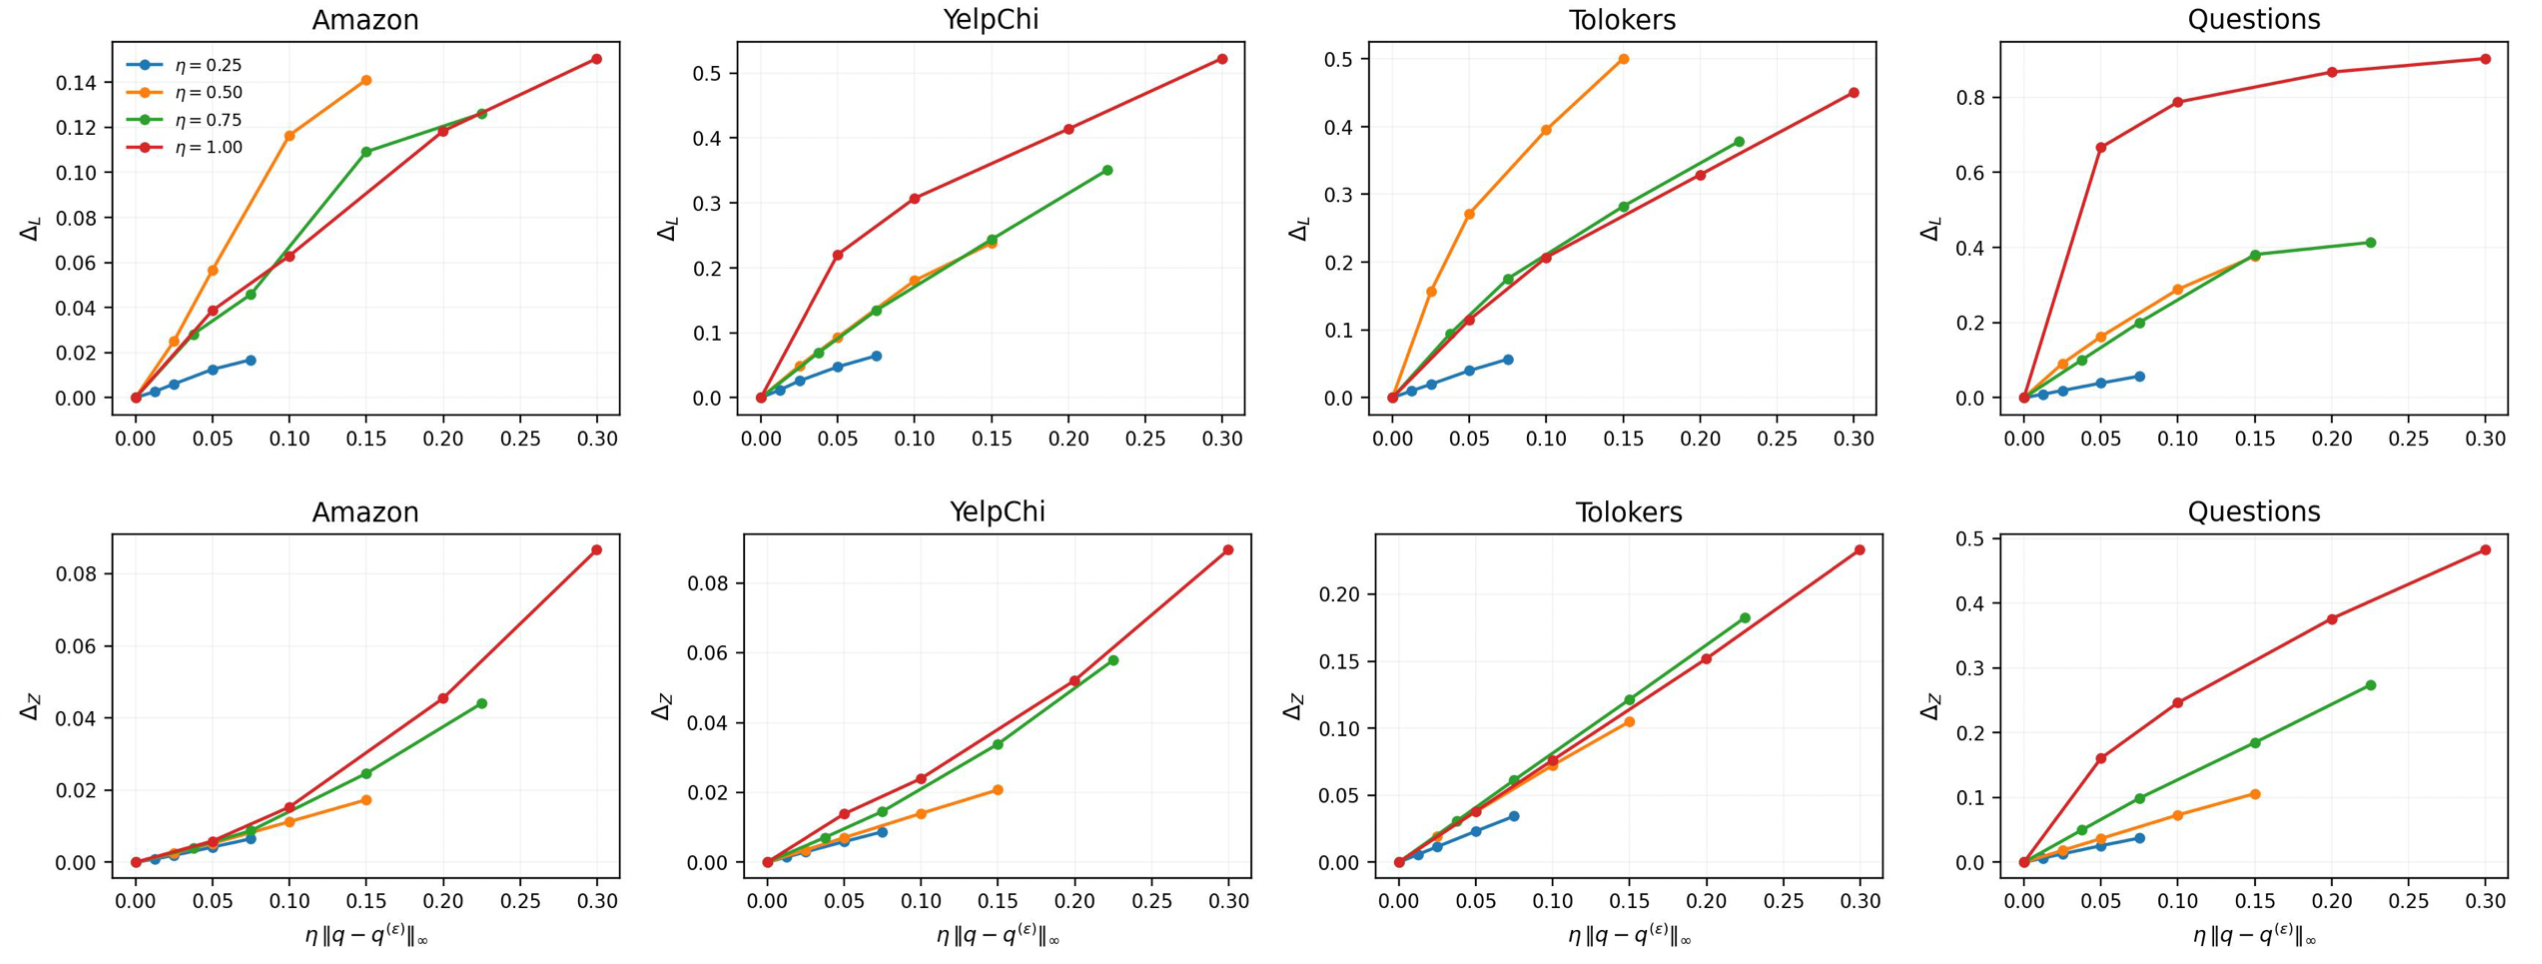
\includegraphics[width=\linewidth]{images/rq3.png}}
\caption{Robustness to edge-calibration errors under different fixed calibration strengths $\eta$.
The horizontal axis denotes the scaled calibration perturbation $\eta\|q-q^{(\epsilon)}\|_\infty$.
The top row plots the operator perturbation $\Delta_L=\|L_\eta(q)-L_\eta(q^{(\epsilon)})\|_2$ and the bottom row plots the normalized representation perturbation $\Delta_Z=\|Z(q)-Z(q^{(\epsilon)})\|_F/\|H^{(0)}\|_F$, averaged over 10 splits.} 
\label{fig:rq3}
% \vspace{-10pt}
\end{figure*}

We analyze the empirical implications of Theorems~\ref{thm:stab} and~\ref{thm:repr} by perturbing the frozen edge-calibration scores $\hat{q}_{uv}$ and its calibration strength while keeping the later training pipeline the same.
First, the learned $\hat{q}$ is kept as the fixed $q$. We then add a small error $\epsilon$ to get a perturbation of $q$, denoted as $q^{(\epsilon)}$.
Specifically, we generate $q^{(\epsilon)}=\mathrm{clip}(q+\Delta_\epsilon,0,1)$ with $\Delta_\epsilon\sim U(-\epsilon,\epsilon)$ drawn i.i.d.\ per non-self-loop edge and vary $\epsilon\in\{0,0.05,0.10,0.20,0.30\}$.
Then, the approximation errors are computed as $\Delta_q=\|q-q^{(\epsilon)}\|_\infty$ after clipping.
We also fix $\eta\in\{0.25,0.50,0.75,1.00\}$. 
Since $\eta$ is fixed within each experiment, the calibration strength mismatch term in Theorem~\ref{thm:stab} vanishes, leaving the operator perturbation controlled by the scaled local calibration error $\eta\,\eloc(q,q^{(\epsilon)})$, which is at most the scaled worst-edge error $\eta\|q-q^{(\epsilon)}\|_\infty$ on the horizontal axis.
This error is also considered in the subsequent robustness analysis of the mapping function $\bm Z$ in Theorem~\ref{thm:repr}.
The plots of the perturbation effects are presented in Fig.~\ref{fig:rq3}.

Figure~\ref{fig:rq3} shows that $\Delta_L$ systematically increases as this quantity grows across all four datasets, with weak calibration remaining in a substantially lower-perturbation regime. 
The curves are not expected to share a common slope, since the theorem gives a perturbation bound rather than an equality and the realized sensitivity also depends on graph normalization and topology. 
Nevertheless, the observed scaling highlights that $\eta$ directly modulates how calibration uncertainty enters the signed propagation operator, which is consistent with the central claim of Theorem~\ref{thm:stab}.

The second row of Fig.~\ref{fig:rq3} further shows that perturbations of the signed operator propagate to the learned spectral representation.
$\Delta_Z$ generally increases with the induced operator error, while remaining markedly smaller than $\Delta_L$ in several settings. 
This behavior indicates that the multi-channel spectral transformation does not amplify the errors from edge-calibration phase, which is highlighted by the vanishing of the gate $\bm g$ in the bound of Theorem~\ref{thm:repr}.
Importantly, these results sharpen the role of soft signing in ESO-GAD. 
The calibration strength $\eta$ is not only a parameter controlling the amount of heterophilic information injected into propagation.
It also provides an explicit robustness mechanism that regulates exposure to errors in the edge-heterophily estimator.
%Thus, ESO-GAD couples edge-semantic exploitation with controlled sensitivity to calibration uncertainty, providing a principled alternative to committing fully to noisy heterophilic estimates.
%Figure~\ref{fig:rq3} therefore offers empirical evidence for the structural perturbation pathway underlying Theorem~1, rather than claiming exact tightness of the theoretical bounds or a universal relationship with downstream accuracy.

\subsubsection{Analysis on KL-regularized spectral gating}
\label{sec:rq6}
In the aggregation gate of Eq.~\eqref{eq:gate}, 
we compare the full ESO-GAD gate with two simplified alternatives: fixed uniform aggregation and learnable aggregation without KL regularization. 
Results are averaged over the same 10 random splits.
As shown in Table~\ref{tab:rq6-main}, Learnable+KL achieves the best AUPRC and AUROC on Amazon, YelpChi, and Questions, while remaining competitive on Tolokers. 
These results indicate that adaptive spectral aggregation is generally preferable to uniform weighting, with KL regularization providing additional benefit over unconstrained gating on most datasets.
%The results further support the role of KL regularization in the coupled optimization of the spectral gate and the learnable signed operator $L_\eta$. 
%While the learnable gate enables dataset-adaptive spectral weighting, the KL term discourages premature concentration on a small subset of channels as $L_\eta$ evolves during training. 
%The small exception on Tolokers suggests that KL regularization is not uniformly beneficial, but rather provides a more robust trade-off between spectral adaptivity and regularization. 
%Overall, the results support KL-regularized learnable gating as an effective balance between spectral adaptivity and stable channel utilization in ESO-GAD.

\begin{table*}[t]
\centering
\caption{Comparison between different aggregator gate choices to produce the representation $\bm Z$ from different filter bands. %The results are reported on 4 datasets over 10 runs with AUPRC and AUROC metrics.
}
\label{tab:rq6-main}
\resizebox{0.85\textwidth}{!}{
\begin{tabular}{lcccccccc}
\hline
& \multicolumn{2}{c}{\textbf{Amazon}}
& \multicolumn{2}{c}{\textbf{YelpChi}}
& \multicolumn{2}{c}{\textbf{Tolokers}}
& \multicolumn{2}{c}{\textbf{Questions}} \\
\textbf{Variant}
& \textbf{AUPRC} & \textbf{AUROC}
& \textbf{AUPRC} & \textbf{AUROC}
& \textbf{AUPRC} & \textbf{AUROC}
& \textbf{AUPRC} & \textbf{AUROC} \\
\hline

Uniform Gate
& 82.80$_{\pm2.11}$
& 93.04$_{\pm1.74}$
& 27.90$_{\pm3.38}$
& 68.58$_{\pm4.32}$
& \underline{40.31}$_{\pm2.41}$
& 73.05$_{\pm1.59}$
& \underline{9.25}$_{\pm1.82}$
& 67.92$_{\pm3.81}$ \\

Learnable, no KL
& \underline{83.06}$_{\pm2.30}$
& \underline{93.68}$_{\pm1.90}$
& \underline{28.17}$_{\pm3.25}$
& \underline{69.14}$_{\pm3.89}$
& \textbf{40.45}$_{\pm2.04}$
& \textbf{73.36}$_{\pm2.20}$
& 9.07$_{\pm1.79}$
& \underline{68.01}$_{\pm3.55}$ \\

Learnable + KL (ESO-GAD)
& \textbf{83.73}$_{\pm1.33}$
& \textbf{94.12}$_{\pm1.37}$
& \textbf{28.87}$_{\pm2.07}$
& \textbf{69.74}$_{\pm2.45}$
& 40.37$_{\pm1.69}$
& \underline{73.18}$_{\pm1.53}$
& \textbf{9.78}$_{\pm1.83}$
& \textbf{68.54}$_{\pm2.55}$ \\

\hline
\end{tabular}
}
\end{table*}

% In the preamble

\subsubsection{Calibration Strength Sensitivity}
We study the impact of the calibration strength $\eta$ on the performance of ESO-GAD by evaluating $\eta\in\{0.25,0.50,0.75,1.00\}$ and adaptive $\eta$ while keeping all other settings fixed.
Figure~\ref{fig:eta-sensitivity} shows that both Amazon and YelpChi favor a moderate strength, with the highest fixed AUPRC among the evaluated values attained at $\eta=0.75$.
Performance does not improve at the reweighting boundary ($\eta=0.5$) but increases for $\eta>0.5$.
Performance subsequently decreases at $\eta=1.0$ on both datasets, suggesting that the estimation errors from the edge calibrator should be controlled properly.
The learned adaptive values also fall near the empirically favorable region, providing evidence that adaptive $\eta$ can recover a competitive calibration value without explicit manual tuning.


\begin{figure}[t]
    \centering
    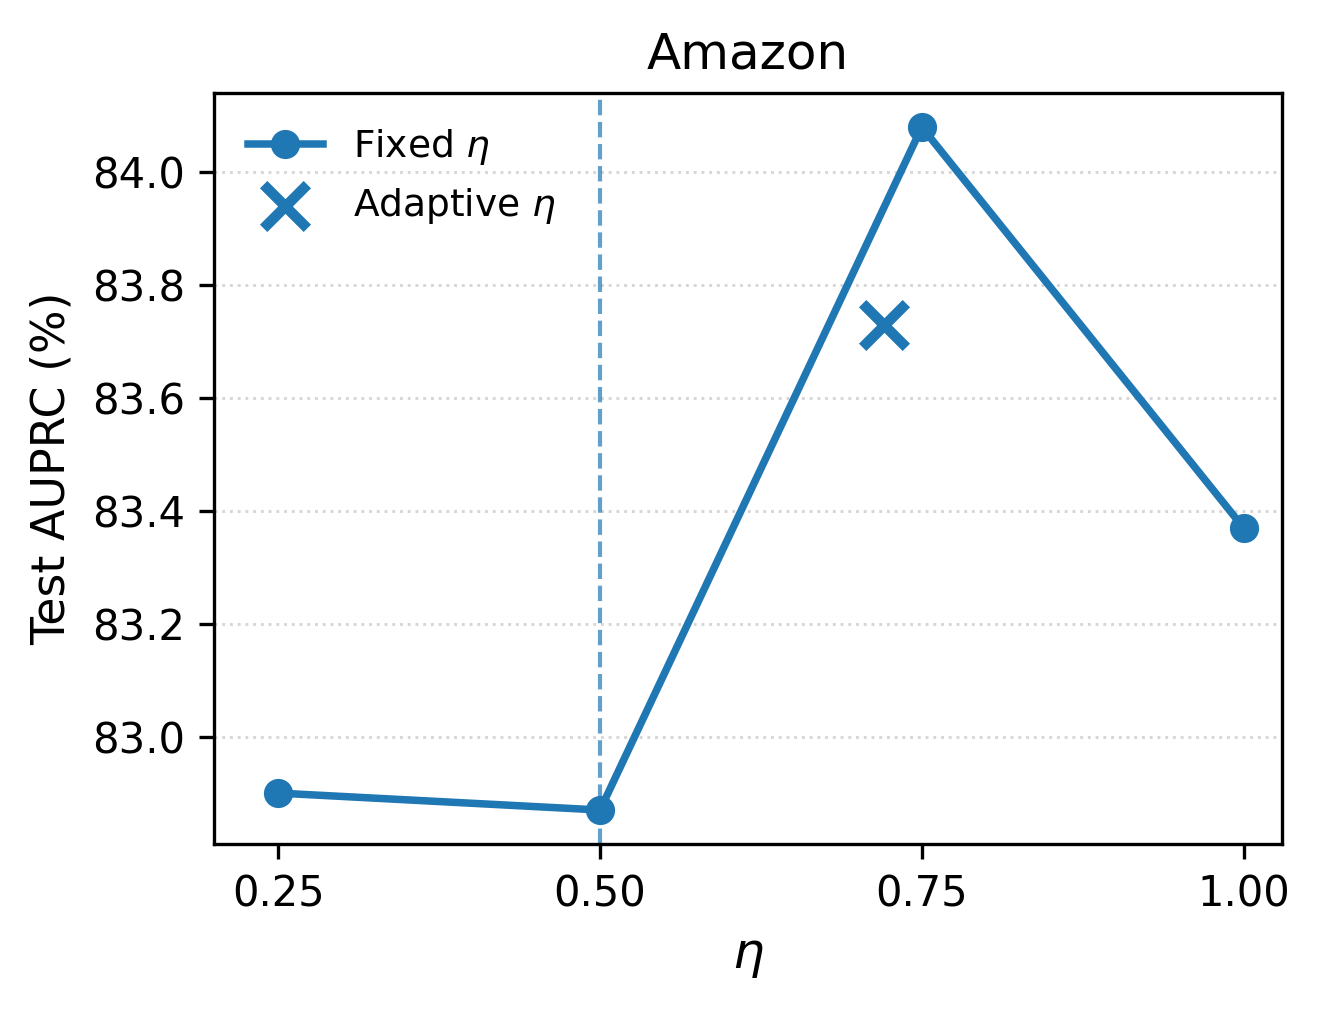
\includegraphics[width=0.48\linewidth]{images/eta_sensitivity_amazon_xlabel_eta.png}
    \hfill
    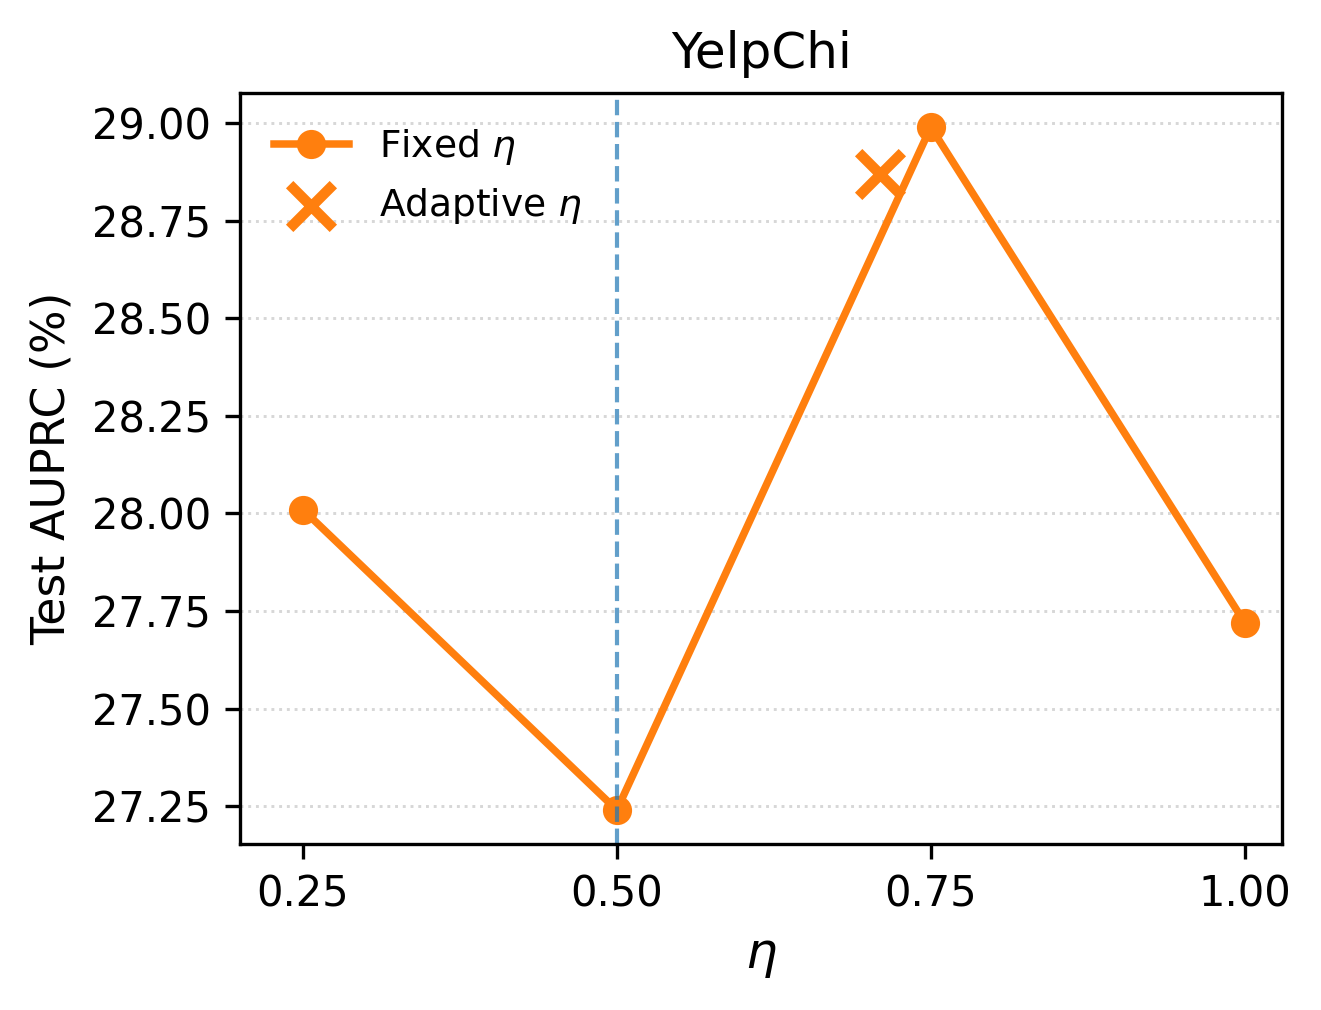
\includegraphics[width=0.48\linewidth]{images/eta_sensitivity_yelpchi_xlabel_eta.png}
    
    \caption{
    Sensitivity to the {calibration strength} $\eta$ on Amazon  and
    YelpChi.
    The line reports test AUPRC under fixed $\eta$, while $\times$ indicates the learned adaptive $\eta$ after the model converges.
    }
    \label{fig:eta-sensitivity}
\end{figure}

\subsubsection{Runtime Analysis}
We compare the training time of ESO-GAD with several spectral methods on a single RTX 3090.
All methods are re-run in the same settings as in Table~\ref{tab:ESO_gad_auroc}.
Reported values are mean end-to-end  training time with 10 runs. For ESO-GAD, we separately report the edge-calibration cost (Phase 1) and signed spectral training cost (Phase 2).

As shown on Table \ref{tab:runtime}, runtime increases with graph size, with all methods remaining lightweight on YelpChi and Amazon but becoming more expensive on T-Finance.
ESO-GAD incurs a clear overhead over BWGNN due to its additional calibration and signed-training stages.
%requiring 7.5/9.9/63.5 s on YelpChi/Amazon/T-Finance, respectively.
In Phase 2, ESO-GAD has to rebuild the operator in Eq.~\eqref{eq:laplacian} after each update of $\eta$, which makes the training time increase in comparison to other spectral baselines.
Nevertheless, this is the trade-off of using an adaptive calibration strength rather than a fixed value.
\begin{table}[t]
\centering
\caption{Mean total training time (s) over 10 seeds.
ESO-GAD is reported with both Phase~1{+}Phase~2 (P1+P2).}
\label{tab:runtime}
\resizebox{\columnwidth}{!}{%
\begin{tabular}{lrrrr}
\hline
Dataset & BWGNN & GHRN & ChiGAD & ESO-GAD $(P1+P2)$ \\
\hline
YelpChi   & 1.2 & 1.3 & 2.6  & 3.2{+}4.2 \ (7.5) \\
Amazon     & 1.0 & 1.4 & 2.5  & 4.4{+}5.6 \ (9.9) \\
T-Finance & 8.2 & 9.8 & 14.8 & 29.7{+}33.7 \ (63.5) \\
\hline
\end{tabular}}
\end{table}



\section{Conclusion}
In this paper, we study the role of edge heterophily in carrying local information for GAD.
%and extend spectral GNNs by introducing edge semantics into the graph operator on which the filter bank is defined.
Motivated by this view, we propose ESO-GAD, which trains an edge calibrator to estimate heterophily probabilities and encodes them into a signed normalized Laplacian $\bm{L}_\eta$, with an adaptive calibration strength $\eta$.
ESO-GAD then applies a Beta-wavelet filter bank to $\bm{L}_\eta$ and combines its channels through a KL-anchored simplex gate to predict anomaly labels.
Under the GADBench protocol, ESO-GAD consistently improves over its unsigned BWGNN backbone and outperforms most baselines on the seven evaluated datasets.
The main drawback is that the signed operator inherits the bias of the edge calibrator, which is frozen before node-level training.
A feasible extension is therefore to relax this separation and update the calibrator jointly with the spectral filters.
Alternative spectral backbones instead of the Beta-wavelet filter are also promising combinations with our proposed signed operator.





%%
%% The next two lines define the bibliography style to be used, and
%% the bibliography file.


\FloatBarrier

% Required by ICML: unnumbered, before the references, not counted in the page limit.
\section*{Impact Statement}
This work involves neither human nor animal subjects, and the authors collected no personal data.
All experiments use publicly available benchmark datasets, obtained and used under their original licenses, in which user
identities are anonymized.
Graph anomaly detection is typically deployed in fraud detection, spam filtering, and risk control, where false positives impose real costs on the individuals flagged.
Although evaluation under deployment conditions is not within the scope of this paper, we note that ESO-GAD should not serve as the sole basis for consequential decisions about individuals, and that any practical use should retain human review.


\bibliography{references}
\bibliographystyle{icml2026} % ICML STYLE

\newpage
\appendix
\onecolumn

The appendix contains three parts: Appendix~\ref{app:proofs} proves Proposition~\ref{prop:valid} and all results of Section~\ref{sec:theory}; Appendix~\ref{app:additional} reports additional experimental results; and Appendix~\ref{app:details} gives the experimental details.

\section{Proofs}\label{app:proofs}
\allowdisplaybreaks
We use the notation of Section~\ref{sec:theory}.
For a fixed pair $(q,\eta)$ we abbreviate $w_{uv}=W^{(\eta)}_{uv}$, $\sigma_{uv}=\sgn(w_{uv})$, $D_u=D^{(\eta)}_{uu}$ and $\bm N=\Db{}^{-1/2}\Wb\Db{}^{-1/2}$, so that $\Lb=\bm I-\bm N$.
For a vector $\bm h$ we write $\bm f=\Db{}^{-1/2}\bm h$, i.e., $f_u=h_u/\sqrt{D_u}$.
Quantities built from a second pair $(q',\eta')$ carry a prime.

\subsection{Proof of Proposition~\ref{prop:valid}}
For the first inequality, by Eq.~\eqref{eq:Wentry},
$|w_{uv}|=\tilde A_{uv}|1-2\eta\hat q_{uv}|\ge0$, and the self-loop
contributes $|1-2\eta\hat q_{uu}|=1$ since $\hat q_{uu}=0$. Hence
$D_u=\sum_v|w_{uv}|\ge1$ for every $u$, uniformly in
$(\eta,\hat q)$, so $\Db\succeq\bm I\succ0$ and $\Db{}^{-1/2}$ exists.

For the second part, we start by expanding $\bm h^{\!\top}\bm h$ using the symmetry of $\Wb$:
\begin{align}
\bm h^{\!\top}\bm h
&=\sum_uD_uf_u^2=\sum_{u,v}|w_{uv}|f_u^2
=\tfrac12\sum_{u,v}|w_{uv}|\bigl(f_u^2+f_v^2\bigr).
\label{eq:pf-energy}
\end{align}
On the other hand, writing $w_{uv}=\sigma_{uv}|w_{uv}|$ gives
\begin{equation}
\bm h^{\!\top}\Db{}^{-1/2}\Wb\Db{}^{-1/2}\bm h
=\sum_{u,v}|w_{uv}|\,\sigma_{uv}f_uf_v.
\label{eq:pf-cross}
\end{equation}
Subtracting Eq.~\eqref{eq:pf-cross} from Eq.~\eqref{eq:pf-energy} and completing the square,
\begin{equation}
\bm h^{\!\top}\Lb\bm h
=\tfrac12\sum_{u,v}|w_{uv}|\bigl(f_u-\sigma_{uv}f_v\bigr)^2\ge0,
\label{eq:pf-lower}
\end{equation}
which is Eq.~\eqref{eq:quadform} and gives $\lambda_{\min}(\Lb)\ge0$.
Adding instead of subtracting,
\begin{equation}
2\Vert\bm h\Vert^2-\bm h^{\!\top}\Lb\bm h
=\tfrac12\sum_{u,v}|w_{uv}|\bigl(f_u+\sigma_{uv}f_v\bigr)^2\ge0,
\label{eq:pf-upper}
\end{equation}
so $\lambda_{\max}(\Lb)\le2$.
No step uses $\eta\le1$, so the statement holds for every $\eta\ge0$.
\hfill$\square$

\subsection{Proof of Theorem~\ref{thm:gauge}}
With $q=\bm t^\star$ and $\eta\in[\tfrac12,1]$, the weight $w_{uv}=\tilde A_{uv}(1-2\eta\tstar_{uv})$ equals $1$ on homophilic edges and $1-2\eta\le0$ on heterophilic ones.
Hence $|w_{uv}|=\tilde A_{uv}\bigl(1-2(1-\eta)\tstar_{uv}\bigr)$, which is the $(u,v)$ entry of $\bm W^{(1-\eta)}(\bm t^\star)$, and $\sigma_{uv}=\sstar_{uv}=\bar y_u\bar y_v$ wherever $w_{uv}\neq0$.
Therefore
\begin{equation}
\bm W^{(\eta)}(\bm t^\star)=\Ys\,\bm W^{(1-\eta)}(\bm t^\star)\,\Ys
\label{eq:pf-gaugeW}
\end{equation}
entrywise.
The degree matrix depends on the absolute values of the weights only, so both sides of Eq.~\eqref{eq:pf-gaugeW} have the same $\bm D$, and $\Ys$ commutes with diagonal matrices.
Multiplying Eq.~\eqref{eq:pf-gaugeW} by $\bm D^{-1/2}$ on both sides gives $\bm N_\eta=\Ys\bm N_{1-\eta}\Ys$ and, since $\Ys^2=\bm I$, statement~(i).
The weights of $\bm W^{(1-\eta)}(\bm t^\star)$ lie in $[0,1]$, and at $\eta=1$ they equal $\tilde A_{uv}$, which is the unsigned operator $\bm L_0$.

For (ii), $\Ys$ is orthogonal, so the two operators are similar and share their spectrum, and $(\Ys\bm M\Ys)^j=\Ys\bm M^j\Ys$ for every $j\ge0$ gives $g(\Ys\bm M\Ys)=\Ys g(\bm M)\Ys$ for every polynomial $g$.

For (iii), $\bm L_{1-\eta}(\bm t^\star)$ is the normalized Laplacian of a graph with non-negative weights and degree matrix $\bm D$, so $\bm L_{1-\eta}(\bm t^\star)\bm D^{1/2}\bm 1=\bm D^{1/2}\bm 1-\bm D^{-1/2}|\bm W|\bm 1=\bm 0$.
Using $\Ys\ys=\bm 1$,
\[
\bm L_\eta(\bm t^\star)\,\bm D^{1/2}\ys
=\Ys\,\bm L_{1-\eta}(\bm t^\star)\,\Ys\bm D^{1/2}\ys
=\Ys\,\bm L_{1-\eta}(\bm t^\star)\,\bm D^{1/2}\bm 1=\bm 0.
\tag*{$\square$}
\]

\subsection{Proof of Theorem~\ref{thm:freq}}
Apply Eq.~\eqref{eq:pf-lower} to $\bm h=\yt=\Db{}^{1/2}\ys$, for which $\bm f=\ys$.
Since $\bar y_u,\bar y_v\in\{-1,+1\}$, for every pair with $w_{uv}\neq0$ we have $(\bar y_u-\sigma_{uv}\bar y_v)^2=4\cdot\mathds{1}[\sigma_{uv}\neq\bar y_u\bar y_v]$, and pairs with $w_{uv}=0$ do not contribute.
Hence
\[
\yt^{\top}\Lb\,\yt=2\sum_{u,v}|w_{uv}|\,\mathds{1}[\sigma_{uv}\neq\sstar_{uv}].
\]
The denominator is $\yt^{\top}\yt=\sum_uD_u\bar y_u^2=\sum_{u,v}|w_{uv}|$.
The ratio is $2\,\Fr_\eta(q)$ by Eq.~\eqref{eq:frustration}.
\hfill$\square$

\subsection{Proof of Corollary~\ref{cor:lift}}
For $\eta\in[0,\tfrac12]$ every weight $w_{uv}=\tilde A_{uv}(1-2\eta q_{uv})$ is non-negative, so an edge with $w_{uv}\neq0$ is frustrated if and only if it is heterophilic.
The numerator of Eq.~\eqref{eq:frustration} is $\sum_{\mathrm{het}}(1-2\eta q_{uv})=H-2\eta S_{\mathrm{het}}$ and the denominator is $\sum_{\mathrm{all}}(1-2\eta q_{uv})=M-2\eta S_{\mathrm{all}}$; self-loops have $q_{uu}=0$, so they add $n$ to $M$ and nothing to $S_{\mathrm{all}}$, and the denominator is at least $n>0$.
At $\eta=0$ this gives $\Fr_0=H/M$.
Differentiating,
\[
\frac{d}{d\eta}\Fr_\eta(q)=\frac{2\,(S_{\mathrm{all}}H-S_{\mathrm{het}}M)}{(M-2\eta S_{\mathrm{all}})^2},
\]
whose sign does not depend on $\eta$ and is negative if and only if $S_{\mathrm{het}}/H>S_{\mathrm{all}}/M$.

For general $\eta$, a heterophilic edge is frustrated if and only if its weight is positive and then contributes $(1-2\eta q_{uv})_+$, while a homophilic edge is frustrated if and only if its weight is negative and then contributes $(2\eta q_{uv}-1)_+$, which gives the expression stated after the corollary.
\hfill$\square$

\subsection{Proof of Corollary~\ref{cor:energy}}
Let $\Lb=\sum_i\lambda_i\bm u_i\bm u_i^{\top}$ and let $\mu_y$ be the probability measure that puts mass $\langle\bm u_i,\yt\rangle^2/\|\yt\|_2^2$ on $\lambda_i$.
By Proposition~\ref{prop:valid} it is supported on $[0,2]$, its mean is $\rho_\eta(q)=2\Fr_\eta(q)$ by Theorem~\ref{thm:freq}, and
\[
E_0=\int\Bigl(1-\frac\lambda2\Bigr)^{2P}d\mu_y(\lambda),\qquad
E_P=\int\Bigl(\frac\lambda2\Bigr)^{2P}d\mu_y(\lambda).
\]
Both integrands are convex, so Jensen's inequality gives $E_0\ge(1-\rho/2)^{2P}$ and $E_P\ge(\rho/2)^{2P}$.
On $[0,2]$ we have $(1-\lambda/2)^{2P}\le1-\lambda/2$ and $(\lambda/2)^{2P}\le\lambda/2$, so $E_0\le1-\rho/2$ and $E_P\le\rho/2$.
Under oracle signs and $\eta\in(\tfrac12,1]$, Theorem~\ref{thm:gauge}(iii) gives $\mu_y=\delta_0$, hence $E_0=1$ and $E_k=0$ for $k\ge1$ because $\mathcal W_k$ contains the factor $(\Lb/2)^k$.
\hfill$\square$

\subsection{Proof of Theorem~\ref{thm:snr}}
\textbf{(a)} By Assumption~\ref{ass:features}, $\bm Z=\bm G\ys\bm\mu^{\top}+\bm G\bm\Xi$.
Row $u$ of $\bm G\bm\Xi$ is the combination $\sum_vG_{uv}\bm\xi_v$ of independent Gaussian vectors, so it is $\mathcal N(\bm 0,\sigma^2\|\bm G_{u\cdot}\|_2^2\bm I)$ and
\[
\frac{\langle\bm z_u,\bm\mu\rangle}{\|\bm\mu\|}\sim\mathcal N\Bigl([\bm G\ys]_u\,\|\bm\mu\|,\;\sigma^2\|\bm G_{u\cdot}\|_2^2\Bigr).
\]
The readout errs when $\bar y_u\langle\bm z_u,\bm\mu\rangle\le0$, which has probability $\Gt\bigl(\bar y_u[\bm G\ys]_u\|\bm\mu\|/(\sigma\|\bm G_{u\cdot}\|_2)\bigr)$.
For $\bm G=\Db{}^{-1}\Wb$,
\[
\bar y_u[\bm G\ys]_u=\frac{\sum_vw_{uv}\bar y_u\bar y_v}{D_u}=\mar_u,
\qquad
\|\bm G_{u\cdot}\|_2=\frac{(\sum_vw_{uv}^2)^{1/2}}{\sum_v|w_{uv}|}=\bigl(\deff_u\bigr)^{-1/2}.
\]

\noindent\textbf{(b)} The self-loop is homophilic with weight $1$ in all three cases.
For the unsigned operator all $\tilde d_u$ weights equal $1$, so $\mar_u=(\tilde d_u-2\tilde h_u\tilde d_u)/\tilde d_u=1-2\tilde h_u$ and $\deff_u=\tilde d_u$.
For oracle pruning the $(1-\tilde h_u)\tilde d_u$ homophilic edges keep weight $1$ and the others weight $0$, so $\mar_u=1$ and $\deff_u=(1-\tilde h_u)\tilde d_u$.
For oracle signing $w_{uv}=\sstar_{uv}$, so $\mar_u=1$ and $\deff_u=\tilde d_u$.
The statement on the class means follows from $[\bm G\ys]_u=\mar_u\bar y_u$: the mean of $\bm z_u$ is $(1-2\tilde h_u)\bm\mu$ for an anomaly and $-(1-2\tilde h_u)\bm\mu$ for a normal node, and averaging over the two classes gives the difference $2(1-\tilde h_a-\tilde h_n)\bm\mu$.

\noindent\textbf{(c)} By Theorem~\ref{thm:gauge} with $\eta=1$, $\bm I-\bm L_1(\bm t^\star)=\Ys(\bm I-\bm L_0)\Ys$, hence $\bm G_s=\Ys\bm G_0\Ys$.
The matrix $\bm I-\bm L_0$ is entrywise non-negative and $g$ has non-negative coefficients, so $\bm G_0\ge0$ entrywise.
Using $\Ys\ys=\bm 1$ and $\bar y_u^2=1$,
\[
\bar y_u[\bm G_s\ys]_u=[\bm G_0\bm 1]_u=\|\bm G_{0,u\cdot}\|_1,
\qquad
\|\bm G_{s,u\cdot}\|_2=\|\bm G_{0,u\cdot}\|_2.
\]
For the unsigned operator, $|\bar y_u[\bm G_0\ys]_u|=\bigl|\sum_vG_{0,uv}\,\bar y_u\bar y_v\bigr|\le\sum_vG_{0,uv}$, with equality if and only if $\bar y_u\bar y_v$ is constant on the support of row $u$.
Because of the self-loops, every power of $\bm I-\bm L_0$ has a positive diagonal, so $u$ belongs to the support of its own row, and equality holds if and only if all nodes of the support have the class of $u$.

\noindent\textbf{(d)} Write $d=\tilde d_u$, $H_u=\tilde h_ud$, and let $S_{\mathrm{het}}$, $S_{\mathrm{hom}}$ be the sums of the scores over the heterophilic and homophilic edges of $u$, $S=S_{\mathrm{het}}+S_{\mathrm{hom}}$, and $S_2$ the sum of the squared scores.
For $\eta<\tfrac12$ all weights are positive, and
\[
\mar_u(\eta)=\frac{(d-2H_u)-2\eta\,(S_{\mathrm{hom}}-S_{\mathrm{het}})}{d-2\eta S},\qquad
\deff_u(\eta)=\frac{(d-2\eta S)^2}{d-4\eta S+4\eta^2S_2}.
\]
Differentiating at $\eta=0$,
\[
\mar_u'(0)=\frac{4}{d^2}\Bigl[S_{\mathrm{het}}(d-H_u)-H_uS_{\mathrm{hom}}\Bigr]
=4\,\tilde h_u(1-\tilde h_u)\bigl(\bar q^{\mathrm{het}}_u-\bar q^{\mathrm{hom}}_u\bigr),
\]
with $\bar q^{\mathrm{het}}_u=S_{\mathrm{het}}/H_u$ and $\bar q^{\mathrm{hom}}_u=S_{\mathrm{hom}}/(d-H_u)$, and $(\deff_u)'(0)=(-4dS+4dS)/d^2=0$.
Since $\snr_u=\mar_u\sqrt{\deff_u}$ and $\deff_u(0)=d$, the claim follows.
\hfill$\square$

\subsection{Proof of Theorem~\ref{thm:optimal}}
Write $\bm h^{(0)}_v=\bar y_v\bm\mu+\bm\xi_v$ and $s_{uv}=\bar y_u\bar y_v$, with $s_{uu}=1$.
Then
\[
\bar y_u\langle\bm z_u,\hat{\bm\mu}\rangle=\|\bm\mu\|\sum_v\vartheta_vs_{uv}+\bar y_u\sum_v\vartheta_v\langle\bm\xi_v,\hat{\bm\mu}\rangle.
\]
Conditionally on $y_u$ and the scores, Assumption~\ref{ass:reliability} gives $\mathbb E[s_{uv}]=1-2p(q_{uv})=c_v$ and $\operatorname{Var}[s_{uv}]=1-c_v^2$, independently across $v$, and the noise terms are independent of the signs with variance $\sigma^2$.
Hence the conditional mean is $\|\bm\mu\|\sum_v\vartheta_vc_v$ and the conditional variance is $\sum_v\vartheta_v^2\bigl(\|\bm\mu\|^2(1-c_v^2)+\sigma^2\bigr)=\sum_v\vartheta_v^2\varsigma_v^2$, which gives the stated form of $\mathcal J$.

\noindent\textbf{(i)} By the Cauchy--Schwarz inequality,
\[
\sum_v\vartheta_vc_v=\sum_v(\vartheta_v\varsigma_v)\frac{c_v}{\varsigma_v}
\le\Bigl(\sum_v\vartheta_v^2\varsigma_v^2\Bigr)^{1/2}\Bigl(\sum_v\frac{c_v^2}{\varsigma_v^2}\Bigr)^{1/2},
\]
with equality if and only if $\vartheta_v\varsigma_v\propto c_v/\varsigma_v$ with a positive factor.

\noindent\textbf{(ii)} For $\bm\vartheta\ge0$ we have $\sum_v\vartheta_vc_v\le\sum_v\vartheta_v(c_v)_+$, with equality if and only if $\vartheta_v=0$ whenever $c_v<0$, and the Cauchy--Schwarz inequality applied to $(c_v)_+$ gives the bound and its equality case.

\noindent\textbf{(iii)} $(\mathcal J^\star)^2-(\mathcal J^\star_+)^2=\|\bm\mu\|^2\sum_{v:\,c_v<0}c_v^2/\varsigma_v^2$, and $c_v<0$ if and only if $p(q_{uv})>\tfrac12$.

\noindent\textbf{(iv)} Let $X=\bar y_u\langle\bm z_u,\hat{\bm\mu}\rangle$ with conditional mean $m>0$ and variance $v$.
Cantelli's inequality gives $\Pr[X\le0]=\Pr[X-m\le-m]\le v/(v+m^2)=1/(1+\mathcal J(\bm\vartheta)^2)$.
\hfill$\square$

\subsection{Proof of Corollary~\ref{cor:slope}}
By Theorem~\ref{thm:optimal}(i) the optimal weights are proportional to $c_v/\varsigma_v^2$ with $\varsigma_v^2=\sigma^2\bigl(1+(\|\bm\mu\|/\sigma)^2(1-c_v^2)\bigr)$, so $\sigma^2c_v/\varsigma_v^2\to c_v$ uniformly in $v$ as $\|\bm\mu\|/\sigma\to0$.
With $p(q)=\eta_0q$ we have $c_v=1-2\eta_0\hat q_{uv}$ for $v\neq u$, and $c_u=1=1-2\eta_0\hat q_{uu}$ because $\hat q_{uu}=0$.
These are the entries of row $u$ of $\bm W^{(\eta_0)}$ by Eq.~\eqref{eq:Wentry}.
\hfill$\square$

\subsection{Proof of Proposition~\ref{prop:e1}}
Fix an edge with descriptor $\bm z$.
By definition, its endpoints are both anomalous, of different classes, or both normal with probabilities $P_{aa}$, $q^\star$, $P_{nn}$, and by Assumption~\ref{ass:sampling} the labeling is independent of $\bm z$ given the classes.
The edge belongs to $\mathcal E_1$ when exactly one endpoint is labeled, and its target is $1$ when that endpoint is anomalous.
If both endpoints are anomalous, this happens with probability $2r_1(1-r_1)$.
If the endpoints differ, the target is $1$ when the anomalous endpoint is labeled and the normal one is not, with probability $r_1(1-r_0)$, and $0$ in the opposite configuration, with probability $r_0(1-r_1)$.
If both endpoints are normal, the target is $0$ with probability $2r_0(1-r_0)$.
Therefore
\begin{align*}
\Pr[t_{uv}=1,\ (u,v)\in\mathcal E_1\mid\bm z]&=r_1\bigl[2(1-r_1)P_{aa}+(1-r_0)q^\star\bigr],\\
\Pr[t_{uv}=0,\ (u,v)\in\mathcal E_1\mid\bm z]&=r_0\bigl[2(1-r_0)P_{nn}+(1-r_1)q^\star\bigr],
\end{align*}
and the ratio is the stated odds.
If $r_1=r_0$ the factors $1-r$ cancel and the odds equal $(2P_{aa}+q^\star)/(2P_{nn}+q^\star)=\iota/(1-\iota)$, because $1-\iota=P_{nn}+\tfrac12q^\star$; hence $\mathbb E[t_{uv}\mid\bm z]=\iota(\bm z)$.
In general each factor $1-r_c$ lies in $[1-r,1]$, so the first bracket lies in $[(1-r)\,2\iota,\,2\iota]$ and the second in $[(1-r)\,2(1-\iota),\,2(1-\iota)]$, which gives the last claim.
\hfill$\square$

\subsection{Proof of Corollary~\ref{cor:camouflage}}
For a normal node, the edges to anomalies are negative and heterophilic and all other edges are positive and homophilic, so every edge is correctly signed and $\mar_u=1$.
For an anomaly, the self-loop is positive and correct, the $\tilde h_u\tilde d_u$ edges to normal nodes are negative and correct, and the remaining $\tilde d_u-1-\tilde h_u\tilde d_u$ edges to other anomalies are negative but homophilic.
All weights have absolute value $1$, so
\[
\mar_u=\frac{1+\tilde h_u\tilde d_u-(\tilde d_u-1-\tilde h_u\tilde d_u)}{\tilde d_u}=2\tilde h_u-1+\frac{2}{\tilde d_u}.
\]
This exceeds the unsigned margin $1-2\tilde h_u$ if and only if $4\tilde h_u>2-2/\tilde d_u$.
\hfill$\square$

\begin{table}[h]
\centering
\caption{Expected number of doubly-labeled edges ($\mathcal E_2$) and singly-labeled edges ($\mathcal E_1$) when $100$ labeled nodes are drawn uniformly, computed from the statistics of Table~\ref{Tab: Dataset statistics} as $|\mathcal E|\tfrac{100\cdot99}{n(n-1)}$ and $|\mathcal E|\tfrac{2\cdot100\,(n-100)}{n(n-1)}$.}
\label{tab:e2size}
\small
\begin{tabular}{lrrrr}
\toprule
Dataset & $n$ & $|\mathcal E|$ & $\mathbb E|\mathcal E_2|$ & $\mathbb E|\mathcal E_1|$ \\
\midrule
Amazon & 11,944 & 4,398,392 & 305.3 & 73,040 \\
YelpChi & 45,954 & 3,846,979 & 18.0 & 16,707 \\
T-Finance & 39,357 & 21,222,543 & 135.6 & 107,575 \\
Tolokers & 11,758 & 519,000 & 37.2 & 8,754 \\
Reddit & 10,984 & 168,016 & 13.8 & 3,032 \\
Weibo & 8,405 & 407,963 & 57.2 & 9,593 \\
Questions & 48,921 & 153,540 & 0.6 & 626 \\
\bottomrule
\end{tabular}
\end{table}

\subsection{Proof of Proposition~\ref{prop:crossfit}}
\textbf{(i)} If $v$ is unlabeled or $v\in\mathcal F_a$, the only fold that contains an endpoint of $(u,v)$ is $\mathcal F_a$, so $\hat q_{uv}=\phi^{(a)}(\vz_{uv})$.
The descriptor $\vz_{uv}$ depends on the graph and the features only.
The model $\phi^{(a)}$ is trained on edges none of whose labeled endpoints lies in $\mathcal F_a$, and the targets of Eq.~\eqref{eq:edge-target} use the labels of the labeled endpoints only, so $\phi^{(a)}$ is a function of the graph, the features and the labels outside $\mathcal F_a$.

\noindent\textbf{(ii)} If $v\in\mathcal F_b$ with $b\neq a$, both folds contain an endpoint, so $\hat q_{uv}=\tfrac12\bigl(\phi^{(a)}+\phi^{(b)}\bigr)(\vz_{uv})$.
Since $u\notin\mathcal F_b$, the training set of $\phi^{(b)}$ contains the edges between $u$ and every neighbor that is unlabeled or labeled outside $\mathcal F_b$, with targets that depend on $y_u$.

For the last claim, a model trained without $\mathcal F_a\cup\mathcal F_b$ uses no label of either fold, so combined with (i) every edge incident to $u$ is scored by models that never use $y_u$.
\hfill$\square$

\subsection{Proof of Theorem~\ref{thm:stab}}
We use two elementary facts.

\begin{lemma}\label{lem:schur}
Let $\bm M$ be symmetric with non-negative entries, and let $\bm x$ have positive entries with $\bm M\bm x\le\delta\bm x$ entrywise. Then $\|\bm M\|_2\le\delta$. Moreover, $\|\bm A\|_2\le\|\,|\bm A|\,\|_2$ for every symmetric $\bm A$, where $|\bm A|$ is the entrywise absolute value.
\end{lemma}
\begin{proof}
For every vector $\bm v$, using $2ab\le a^2+b^2$ with $a=|v_u|/x_u$, $b=|v_w|/x_w$ and the symmetry of $\bm M$,
\[
|\bm v^{\top}\bm M\bm v|\le\sum_{u,w}M_{uw}x_ux_w\frac{|v_u|}{x_u}\frac{|v_w|}{x_w}
\le\sum_u\frac{v_u^2}{x_u^2}\,x_u\sum_wM_{uw}x_w\le\delta\|\bm v\|_2^2.
\]
The second claim follows from $|\bm v^{\top}\bm A\bm v|\le|\bm v|^{\top}|\bm A|\,|\bm v|$.
\end{proof}

Write $\bm L'-\bm L=\bm N-\bm N'=\bm T_1+\bm T_2$ with
\[
\bm T_1=\bm D^{-1/2}(\bm W-\bm W')\bm D^{-1/2},\qquad
\bm T_2=\bm D^{-1/2}\bm W'\bm D^{-1/2}-\bm N'.
\]

\emph{Bound on $\bm T_1$.}
Let $\bm M=\bm D^{-1/2}|\bm W-\bm W'|\bm D^{-1/2}$ and $\bm x=\bm D^{1/2}\bm 1$.
Then $(\bm M\bm x)_u=D_u^{-1/2}\sum_v|w_{uv}-w'_{uv}|\le\delta\,x_u$ by the definition of $\delta$, and Lemma~\ref{lem:schur} gives $\|\bm T_1\|_2\le\|\bm M\|_2\le\delta$.

\emph{Bound on $\bm T_2$.}
Let $\bm R=\bm D^{-1/2}\bm D'^{1/2}$, a diagonal matrix with entries $r_u=\sqrt{D'_u/D_u}$.
Then $\bm D^{-1/2}\bm W'\bm D^{-1/2}=\bm R\bm N'\bm R$ and
\[
\bm T_2=(\bm R-\bm I)\bm N'\bm R+\bm N'(\bm R-\bm I).
\]
Since $|\sqrt x-1|\le|x-1|$ for $x\ge0$ and $\bigl||w'_{uv}|-|w_{uv}|\bigr|\le|w'_{uv}-w_{uv}|$,
\[
|r_u-1|\le\frac{|D'_u-D_u|}{D_u}\le\frac{\sum_v|w_{uv}-w'_{uv}|}{D_u}\le\delta,
\]
so $\|\bm R-\bm I\|_2\le\delta$ and $\|\bm R\|_2\le1+\delta$.
Proposition~\ref{prop:valid} gives $\|\bm N'\|_2\le1$.
Hence $\|\bm T_2\|_2\le\delta(1+\delta)+\delta$, and $\|\bm L-\bm L'\|_2\le3\delta+\delta^2$.

\emph{Bound on $\delta$.}
By Eq.~\eqref{eq:Wentry},
\[
|w_{uv}-w'_{uv}|=2\tilde A_{uv}\,|\eta q_{uv}-\eta'q'_{uv}|
\le2\tilde A_{uv}\bigl(\eta\,|q_{uv}-q'_{uv}|+|\eta-\eta'|\,q'_{uv}\bigr).
\]
Summing over $v$ and dividing by $D_u\ge\gamma\tilde d_u$ gives $\sum_v|w_{uv}-w'_{uv}|/D_u\le\tfrac2\gamma\bigl(\eta\,\bar e_u+|\eta-\eta'|\,\tilde d_u^{-1}\sum_v\tilde A_{uv}q'_{uv}\bigr)$, and taking the maximum over $u$ gives the claim.

\emph{The degree-dependent constant.}
For comparison, bounding the three terms of the decomposition $\bm L'-\bm L=\bm D^{-1/2}(\bm W-\bm W')\bm D^{-1/2}+(\bm D^{-1/2}-\bm D'^{-1/2})\bm W'\bm D^{-1/2}+\bm D'^{-1/2}\bm W'(\bm D^{-1/2}-\bm D'^{-1/2})$ by $\|\bm W-\bm W'\|_2\le2\eps\dmax$, $\|\bm D^{-1/2}-\bm D'^{-1/2}\|_2\le\eps\dmax$ and $\|\bm W'\|_2\le\dmax$, with $\eps=\eta\|q-q'\|_\infty+|\eta-\eta'|$ and $\dmax=\max_u\tilde d_u$, gives $\|\bm L-\bm L'\|_2\le2\dmax(1+\dmax)\,\eps$.
This is the constant mentioned after Theorem~\ref{thm:stab}.
\hfill$\square$

\subsection{Proof of Theorem~\ref{thm:brier}}
We use the decomposition $\bm N-\bm N'=\bm T_1+\bm T_2$ of the previous proof with $\eta'=\eta$, and write $\delta_u=|D'_u-D_u|/D_u\le\delta$.

\emph{Bound on $\bm T_1$.}
Since $|w_{uv}-w'_{uv}|=2\eta\tilde A_{uv}|q_{uv}-q'_{uv}|$, $D_u\ge\gamma\tilde d_u$ and $D_v\ge1$,
\[
\|\bm T_1\|_F^2=\sum_{u,v}\frac{(w_{uv}-w'_{uv})^2}{D_uD_v}
\le\frac{4\eta^2}{\gamma}\sum_u\frac{1}{\tilde d_u}\sum_v\tilde A_{uv}(q_{uv}-q'_{uv})^2=\frac{4\eta^2}{\gamma}\,\mathcal B(q,q').
\]

\emph{Bound on $\bm T_2$.}
The entries of $\bm T_2=\bm R\bm N'\bm R-\bm N'$ are $N'_{uv}(r_ur_v-1)$, and
$|r_ur_v-1|\le|r_u-1|\,r_v+|r_v-1|\le\delta_u(1+\delta)+\delta_v$.
The rows of $\bm N'$ have squared norm at most $1$, because $|w'_{uv}|\le D'_v$ gives
$\sum_vw'^2_{uv}/(D'_uD'_v)\le\sum_v|w'_{uv}|/D'_u=1$, and the same holds for its columns by symmetry.
Using $(a+b)^2\le2a^2+2b^2$,
\[
\|\bm T_2\|_F^2\le2(1+\delta)^2\sum_u\delta_u^2\sum_vN'^2_{uv}+2\sum_v\delta_v^2\sum_uN'^2_{uv}
\le2\bigl[(1+\delta)^2+1\bigr]\sum_u\delta_u^2\le2(2+\delta)^2\sum_u\delta_u^2.
\]
Finally $\delta_u\le\sum_v|w_{uv}-w'_{uv}|/D_u\le\tfrac{2\eta}{\gamma}\bar e_u$, and $\bar e_u^2\le b_u$ by Jensen's inequality, so $\sum_u\delta_u^2\le\tfrac{4\eta^2}{\gamma^2}\mathcal B(q,q')$.

Combining the two bounds with $\gamma\le1$,
\[
\|\bm N-\bm N'\|_F\le\frac{2\eta}{\sqrt\gamma}\sqrt{\mathcal B}+\frac{2\eta}{\gamma}\sqrt2\,(2+\delta)\sqrt{\mathcal B}
\le\frac{2\eta}{\gamma}\Bigl(1+\sqrt2\,(2+\delta)\Bigr)\sqrt{\mathcal B(q,q')}.
\tag*{$\square$}
\]

\subsection{Proof of Theorem~\ref{thm:repr}}
Abbreviate $\bm L=\bm L_\eta(q)$ and $\bm L'=\bm L_\eta(q')$.
Write $\Wk(\bm L)=\kappa_k\prod_{m=1}^{P}\bm F_m$, with
$\bm F_m=\bm L/2$ for $m\le k$ and $\bm F_m=\bm I-\bm L/2$ otherwise, and define $\bm F'_m$ from $\bm L'$ similarly.
By Proposition~\ref{prop:valid} every factor satisfies
$\Vert\bm F_m\Vert_2,\Vert\bm F'_m\Vert_2\le1$, while
$\Vert\bm F_m-\bm F'_m\Vert_2=\tfrac12\Vert\bm L-\bm L'\Vert_2$ in both cases.
Telescoping the product and bounding the untouched factors by $1$,
\begin{equation}
\Bigl\Vert\prod_m\bm F_m-\prod_m\bm F'_m\Bigr\Vert_2
\le\sum_{m=1}^{P}\Vert\bm F_m-\bm F'_m\Vert_2
=\tfrac{P}{2}\Vert\bm L-\bm L'\Vert_2.
\label{eq:pf-prod}
\end{equation}
Hence
\begin{equation}
\Vert\Wk(\bm L)-\Wk(\bm L')\Vert_2\le\Lambda_k\Vert\bm L-\bm L'\Vert_2
\label{eq:pf-kernel}
\end{equation}
with $\Lambda_k=\tfrac12P\kappa_k$, and since
$\Vert\bm M\bm H^{(0)}\Vert_F\le\Vert\bm M\Vert_2\Vert\bm H^{(0)}\Vert_F$,
\begin{equation}
\Vert\bm H_k-\bm H'_k\Vert_F
\le\Lambda_k\Vert\bm L-\bm L'\Vert_2\Vert\bm H^{(0)}\Vert_F.
\label{eq:pf-chan}
\end{equation}
Since $\bm Z$ concatenates the blocks $\sqrt{g_k}\bm H_k$, the
squared Frobenius norm is block-additive, and $\sum_kg_k=1$ gives
\begin{equation}
\Vert\bm Z(q)-\bm Z(q')\Vert_F^2
=\sum_{k=0}^{P}g_k\Vert\bm H_k-\bm H'_k\Vert_F^2
\le\max_k\Vert\bm H_k-\bm H'_k\Vert_F^2.
\label{eq:pf-gate}
\end{equation}
The bound is uniform over the simplex, so it holds for every value of $\bm g$ during training.
Combining Eq.~\eqref{eq:pf-gate} with Eq.~\eqref{eq:pf-chan} and Eq.~\eqref{eq:stabjoint} at $\eta'=\eta$, for which $\delta\le2\eta\,\eloc(q,q')/\gamma$, yields Eq.~\eqref{eq:stabZ}.
\hfill$\square$

\begin{lemma}[Frobenius Lipschitz continuity of the kernels]\label{lem:frob}
Let $\bm L,\bm L'$ be symmetric with spectra in $[0,2]$ and let $f$ be Lipschitz on $[0,2]$ with constant $\ell$. Then $\|f(\bm L)-f(\bm L')\|_F\le\ell\,\|\bm L-\bm L'\|_F$. In particular, $\|\Wk(\bm L)-\Wk(\bm L')\|_F\le\sup_{\lambda\in[0,2]}|\mathcal W_k'(\lambda)|\cdot\|\bm L-\bm L'\|_F$.
\end{lemma}
\begin{proof}
Let $\bm L=\bm U\operatorname{diag}(\lambda_i)\bm U^{\top}$ and $\bm L'=\bm V\operatorname{diag}(\lambda'_j)\bm V^{\top}$ with orthogonal $\bm U,\bm V$, and $\bm C=\bm U^{\top}\bm V$.
The $(i,j)$ entry of $\bm U^{\top}\bigl(f(\bm L)-f(\bm L')\bigr)\bm V$ is $\bigl(f(\lambda_i)-f(\lambda'_j)\bigr)C_{ij}$, and that of $\bm U^{\top}(\bm L-\bm L')\bm V$ is $(\lambda_i-\lambda'_j)C_{ij}$.
The Frobenius norm is invariant under orthogonal transformations, so
\[
\|f(\bm L)-f(\bm L')\|_F^2=\sum_{i,j}\bigl(f(\lambda_i)-f(\lambda'_j)\bigr)^2C_{ij}^2
\le\ell^2\sum_{i,j}(\lambda_i-\lambda'_j)^2C_{ij}^2=\ell^2\|\bm L-\bm L'\|_F^2.\qedhere
\]
\end{proof}

\subsection{Proof of Corollary~\ref{cor:misaligned}}
For $q=\bm t^\star$ and $\eta\in(\tfrac12,1]$ the homophilic edges have weight $1$ and the heterophilic ones have absolute weight $2\eta-1$, so $D^\star_{uu}=\tilde d_u\bigl(1-2(1-\eta)\tilde h_u\bigr)$ and $\gamma^\star=1-2(1-\eta)\max_u\tilde h_u\ge2\eta-1>0$.
Theorem~\ref{thm:stab} with $\bm L=\bm L^\star$, $\bm L'=\hat{\bm L}$ and $\eta'=\eta$ gives $\|\hat{\bm L}-\bm L^\star\|_2\le3\delta+\delta^2$ with $\delta\le2\eta\,\eloc(\hat q,\bm t^\star)/\gamma^\star$.

By Theorem~\ref{thm:gauge}(iii), $\bm L^\star\yt^\star=\bm 0$, hence $\mathcal W_0(\bm L^\star)\yt^\star=\kappa_0(\bm I-\bm L^\star/2)^P\yt^\star=\kappa_0\yt^\star$, whose $u$-th entry is $\kappa_0\sqrt{D^\star_{uu}}\,\bar y_u$.
Let $\bm r=\mathcal W_0(\hat{\bm L})\yt^\star$ and let $\mathcal M$ be the set of nodes at which $r_u$ does not have the sign of $\bar y_u$.
For $u\in\mathcal M$ we have $|r_u-\kappa_0\sqrt{D^\star_{uu}}\,\bar y_u|\ge\kappa_0\sqrt{D^\star_{uu}}$, so by Eq.~\eqref{eq:pf-kernel},
\[
\kappa_0^2\sum_{u\in\mathcal M}D^\star_{uu}\le\bigl\|\bigl(\mathcal W_0(\hat{\bm L})-\mathcal W_0(\bm L^\star)\bigr)\yt^\star\bigr\|_2^2
\le\Lambda_0^2\,(3\delta+\delta^2)^2\sum_uD^\star_{uu}.
\]
Dividing by $\kappa_0^2\sum_uD^\star_{uu}$ and using $\Lambda_0/\kappa_0=P/2$ gives the claim.
\hfill$\square$

\subsection{Numerical checks}\label{app:numerical}
Every identity and bound of Section~\ref{sec:theory} was checked numerically on random two-class graphs with random score vectors and $\eta\in[0,1.6]$.
The spectral inclusion of Proposition~\ref{prop:valid} holds for every sampled $\eta$, the identities of Theorems~\ref{thm:gauge}, \ref{thm:freq} and~\ref{thm:snr}(a) and the gap formula of Theorem~\ref{thm:optimal}(iii) hold to machine precision, and Proposition~\ref{prop:e1} is reproduced by simulation under uniform and class-dependent labeling.
No bound was violated; the largest observed ratio between the left and right sides was $0.16$ for Theorem~\ref{thm:stab}, $0.06$ for Theorem~\ref{thm:brier} and $0.06$ for Theorem~\ref{thm:repr}.

\section{Additional Experiment Results}\label{app:additional}
\begin{table*}[t]
\caption{Results with mean $\pm$ std on seven real-world datasets in terms of Recall@K (RecK).
The bold and underlined values denote the best and second-best results, respectively.}
\centering
\setlength{\tabcolsep}{5.5pt}
\renewcommand{\arraystretch}{1.08}

\resizebox{\textwidth}{!}{%
\begin{tabular}{lccccccc}
\toprule
Methods
& Amazon
& YelpChi
& T-Finance
& Toloker
& Reddit
& Weibo 
& Questions \\
\midrule

% Group 1: General GNN baselines
GAT
& \val{77.07}{1.74}
& \second{28.09}{3.41}
& \val{36.16}{10.32}
& \val{35.10}{1.82}
& \val{6.47}{2.31}
& \val{70.21}{4.58}
& \val{10.92 }{0.97}\\

GCN
& \val{36.89}{2.62}
& \val{17.00}{3.06}
& \val{60.51}{7.46}
& \val{33.40}{3.54}
& \val{6.23}{2.21}
& \best{79.22}{4.29}
& \val{9.76}{1.28}\\

GraphSAGE
& \val{46.68}{5.26}
& \val{23.76}{4.18}
& \val{18.59}{7.57}
& \val{34.97}{2.54}
& \val{5.15}{1.93}
& \val{60.64}{8.95}
& \val{11.44}{1.48}\\

\midrule

% Group 2: Graph fraud detection baselines
PCGNN
& \val{78.03}{1.53}
& \val{27.82}{3.82}
& \val{63.90}{6.27}
& \val{34.23}{1.56}
& \val{3.01}{2.13}
& \val{65.08}{6.60}
& \val{10.14}{4.11}\\

ConsisGAD
& \val{77.50}{2.74}
& \val{25.85}{3.58}
& \best{74.53}{6.98}
& \val{34.68}{1.64}
& \val{4.94}{1.53}
& \val{49.75}{3.46}
& \val{10.50}{2.83}\\

GAGA
& \val{77.98}{1.05}
& \val{18.23}{3.56}
& \val{60.63}{17.45}
& \val{28.42}{3.72}
& \val{3.56}{1.56}
& \val{36.72}{11.60}
& \val{2.87}{0.86}\\

\midrule

% Group 3: Main comparison methods
BWGNN
& \val{77.85}{1.72}
& \val{26.48}{3.06}
& \val{64.86}{11.67}
& \val{35.31}{3.15}
& \val{5.95}{1.43}
& \val{75.14}{3.52}
& \val{10.90}{3.41}\\

ChiGNN
& \second{78.34}{1.62}
& \val{26.40}{3.79}
& \val{63.65}{7.29}
& \val{35.49}{2.66}
& \val{4.94}{2.11}
& \val{58.41}{6.68}
& \val{10.64}{3.68}\\

GHRN
& \val{77.63}{1.40}
& \val{26.70}{3.30}
& \val{68.12}{3.78}
& \second{36.17}{3.06}
& \val{6.26}{1.39}
& \val{72.39}{2.61}
& \val{11.13}{3.51}\\

AMNet
& \val{77.81}{2.36}
& \val{26.66}{4.33}
& \val{65.92}{5.85}
& \val{30.45}{1.90}
& \val{6.78}{1.50}
& \val{62.10}{4.44}
& \val{12.72}{2.76}\\

SEC-GFD
& \val{76.93}{4.31}
& \val{27.44}{2.33}
& \val{63.14}{7.78}
& \val{35.69}{2.80}
& \val{5.80}{1.79}
& \val{75.50}{3.42}
& \second{11.61}{1.75}\\

DSGAD
& \val{77.12}{2.59}
& \val{25.62}{3.10}
& \val{70.74}{4.23}
& \val{34.05}{2.54}
& \second{7.24}{2.86}
& \val{76.29}{3.34}
& \val{10.89}{3.39}\\

\midrule

% Group 4: Proposed method
\textbf{ESO-GAD (ours)}
& \best{79.33}{1.41}
& \best{32.41}{3.45}
& \second{72.43}{3.43}
& \best{40.97}{1.25}
& \best{7.98}{1.49}
& \second{78.89}{1.70}
& \best{15.59}{1.86}\\

\bottomrule
\end{tabular}%
}


\label{tab:ESO_gad_reck}
\end{table*}

We further report Recall@K (RecK) under the same seven-dataset evaluation setting as the AUROC and AUPRC results in Tables~\ref{tab:ESO_gad_auroc} and~\ref{tab:ESO_gad_auprc}.
ESO-GAD achieves the best RecK on five of the seven datasets, including Amazon, YelpChi, Tolokers, Reddit, and Questions.
Our method ranks second on T-Finance and Weibo. The gains are particularly pronounced on YelpChi, Tolokers, and Questions, where ESO-GAD improves over the strongest competing method.
This trend is broadly consistent with Tables~\ref{tab:ESO_gad_auroc} and~\ref{tab:ESO_gad_auprc}, where ESO-GAD also demonstrates strong performance across AUROC and AUPRC, indicating that its improvements extend beyond ranking-based aggregate metrics to retrieving anomalous nodes among the top-ranked predictions.
Although ConsisGAD and GCN achieve slightly higher RecK on T-Finance and Weibo, respectively, ESO-GAD remains competitive on both datasets, supporting the overall robustness of the signed spectral operator across different evaluation criteria.
\section{Experiment Details}\label{app:details}

The implementation details of ESO-GAD are summarized in Table~\ref{tab:hyperparameters}.
In Phase 1, the edge calibrator, a two-layer MLP, is trained for 150 epochs using Adam with a learning rate of $10^{-2}$.
In Phase 2, both the encoder $\psi$ and classifier $\omega$ use two-layer MLPs with hidden dimensions in $\{16,32,64\}$, while the Beta-wavelet order is selected from $\{2,3\}$ and the KL regularization weight $\alpha$ from $\{0.001,0.01,0.1\}$. Phase 2 is also optimized using Adam with a learning rate of $10^{-2}$.
The number of training epochs in Phase 2 follows the GADBench setting.
All of the experiments are tested on a single RTX 3090.

\begin{table}[h]
\centering
\small
\caption{Key hyperparameters of ESO-GAD.}
\label{tab:hyperparameters}
\begin{tabular}{@{}p{1.0cm}p{3.5cm}p{2.8cm}@{}}
\hline
Phase & Hyperparameters & Value \\
\hline
Phase 1
        & Number of folds $K$  & $\{3,5,8\}$ \\
        & Number of layers in $\phi$ & 2 \\
        & Hidden dimension $d_e$ of $\phi$& $\{16,32,64\}$ \\
        & Optimizer & Adam with $lr=10^{-2}$ \\
        & Epochs & 150 \\
\hline
Phase 2 & Wavelet order $P$ & $\{2,3\}$ \\
        & Number of layers in $\psi, \omega$ & 2 \\
        & Hidden dimension $d_h$ of $\psi, \omega$& $\{16,32,64\}$ \\
        & $\alpha$ & $\{0.001,0.01,0.1\}$ \\
        & Optimizer & Adam with $lr=10^{-2}$ \\
\hline
\end{tabular}
\vspace{2pt}
\end{table}

%% Uncomment if the appendices cite references.  Running BibTeX on supp.tex
%% with no \cite commands present produces an empty bibliography.


\end{document}
